\documentclass[12pt,a4paper,twoside]{book}
\usepackage[german,english]{babel}
\usepackage[T1]{fontenc} 
\usepackage[latin1]{inputenc}
\usepackage{amsfonts}
\usepackage{amsmath}
\usepackage{latexsym}
\usepackage{amssymb}
\usepackage{epsfig}
\usepackage{moreverb}
\usepackage{rotating}
\usepackage{enumerate}
\usepackage{graphics, graphicx,wrapfig}
\usepackage{fancybox}
\usepackage{picinpar,varioref,floatflt}
\usepackage{ae}
\usepackage{longtable}
\usepackage{textcomp}
\usepackage{float}
\usepackage{url}
\usepackage{unizhdt}
\usepackage{pdflscape}
\usepackage{eurosym}
\usepackage[numbers]{natbib}
\usepackage{hyperref}

% custom packages
\usepackage{pifont} % checkmark and xmark symbols

% commands
\newcommand{\cmark}{\ding{51}}%
\newcommand{\xmark}{\ding{55}}%


%%%%%%%%%%%%%%%%%%%%%%%%%%%%%%%%%%%%%%%%%%%%%%%%%%

% Define the language of the diploma thesis
\selectlanguage{english}
%\selectlanguage{german}

\pagestyle{headings}

\begin{document}

%%%%%%%%%%%%%%%%%%%%%%%%%%%%%%%%%%%%%%%%%%%%%%%%%%

% Define the author printed on the cover page
\author{Bachmann Simon \\ Brasser Claudio \\ Bucher Michael \\ Spielmann Nicolas }
% Define the city and country of the author
\authorcity{Z\"urich, Switzerland}
% Define the student IDs (Matrikelnummer)
\studentid{14-709-893, }
% Define the title with optional subtitle
\title{Design and Prototypical Implementation of Blockchain Ticketing}
% Define the supervisors
\supervisors{Sina Rafati}
% Define the submission date
\submissiondate{\today}

%%%%%%%%%%%%%%%%%%%%%%%%%%%%%%%%%%%%%%%%%%%%%%%%%%

% Make the title page
\maketitle

% Make the imprint on the back of the cover page
\makeimprint

\pagenumbering{roman}

% Include the files of the diploma thesis
%\cleardoublepage
\chapter*{Abstract}
\addcontentsline{toc}{chapter}{Abstract}

\selectlanguage{german}

Das ist die Kurzfassung...



\selectlanguage{english}
% author: Simon Bachmann

The ticketing industry is and has long been subject to counterfeiting and profiteering. The secondary market for high demand events attracts ticket scalpers, that hoard tickets and try to sell them at prices well above the initial value. This can be seen as a normal market force, that allows quick movers to make a profit. However, it is a concern for many artists and organizers who lose control over their ticket pricing and distribution. For example, Ed Sheeran's Benefit Concert at Albert Hall (UK) in 2017 for the Teenage Cancer Trust was abused for heavy profiteering where tickets with a face value of 75 pounds have been resold for up to 2330 pounds \cite{ed-sheeran-concert-ticket-prices}. Beyond the reputation problem and fairness concern, the secondary market is also problematic due to fraud. Tickets are often fake or have already been used rendering them invalid. 

Blockchain technology offers an opportunity to remedy these issues. In this project an open and decentralized platform for distributing event tickets and regulating the aftermarket is designed, implemented and evaluated. The system operates through smart contracts on the Ethereum blockchain, enabling users to verify the validity of tickets for a given event, ending counterfeit tickets and allowing the secure resale of tickets based on the organizers pricing to avoid ticket scalping. Furthermore, a mechanism to help users detect fraudulent events is discussed. Also, a system that invalidates tickets in a fast and efficient manner is designed and implemented.
%\cleardoublepage
\chapter*{Acknowledgments}
\addcontentsline{toc}{chapter}{Acknowledgments}

We would like to express our sincerest gratitude to our supervisor Sina Rafati for providing invaluable feedback and support in the process of our master project. We would also like to thank Dr. Thomas Bocek for sharing his deep knowledge related to BC technologies and their application. Last, we would like to thank Prof. Dr. Burkhard Stiller for the opportunity to realize our master project at the Communication Systems Group at the University of Zurich.


\tableofcontents

\cleardoublepage
\pagenumbering{arabic}
\chapter{Introduction}\label{chapter:introduction}

\section{Security Risks and Attack Vectors}\label{section:security-risks}

The following sections describe the challenges and attack vectors when building a decentralized ticketing platform.

% author: Simon Bachmann

\subsection{Front Running}\label{subsection:front-running}

Every transaction on a public blockchain is visible to everybody in the network. However, transactions are only considered finalized when they are accepted by a miner and included in a block. The time of publishing a transaction and time of finalization depends on the amount of transaction fees a user is willing to pay. If the network is clogged with unfinalized transactions, it is possible to get a transaction validated with higher transaction fees because miners want to maximize profit and generally include the transactions that offer the highest fees. This leads to the problem that one transaction can be finalized before some other transaction that was published beforehand. 

An initial coin offering (ICO) is a funding mechanism where investors send tokens to a SC. These funds can then be used by the project team to develop the promised platform or service. In return the investors receive a platform specific token that can be used to consume the service. For some ICOs the maximal amount of funding is limited. If that is the case, investors pay high gas fees to have their transaction confirmed quickly. In the past, this has led to a lot of frustration of investors because transaction fees have spiked disproportionately high compared to the average transaction fees when no popular ICO is taking place \cite{bat-ico-tx-fees} \cite{ico-paradox}.

Since event tickets are in many aspects similar to ICOs tokens such as their limited availability, the same problem occurs. When the demand for tickets exceeds its supply, buyers will try to pay higher transaction fees in order to obtain a ticket before someone else. This might also result in disproportionately high transaction fees. 

\subsection{Random Number Manipulation}\label{subsection:random-number-manipulation}
Since the distribution of the tickets has to be fair, it is needed to use a random number as a seed for the lottery of the tickets. This random number has to be the same for all the nodes in the blockchain. One way of achieving such a random number generation, is the usage of the hash of a block n-blocks after the current block in the chain. This introduces the problem, that a miner may not publish the block, whenever the random number is not in his favour. 

This stated problem can be addressed by ensuring the reward for mining the block is higher than the reward of cheating the lottery. 

% author: Michael Bucher

\subsection{Ticket Invalidation}\label{subsection:ticket-invalidation}

When a guest enters with a valid ticket, this ticket somehow has to be marked as used, in order to prevent it from being used multiple times. To change the state of a ticket on the BC a transaction has to be sent and this transaction is put in a queue to be mined and validated. This takes some time and how long it takes depends on how much GAS is paid for this transaction. During this time it could be possible for a guest that has just entered the event to offer his ticket for sale and attach a relatively high GAS fee to the transaction. This high GAS fee would then lead to the ticket being transferred very fast. While the transaction, that marks the ticket as used, is not yet mined, the new owner of this ticket could enter the event and the ticket would have been used twice.

\subsection{Identity Fraud}\label{subsection:identity-fraud}
michi
TODO: if the form of identity is weakly linked to a human such as a mobile phone number -> a scalper can buy prepaid sim cards and sell sim cards on ebay
\subsection{Fraudulent Events}\label{subsection:fraudulent-events}
claudio
TODO: no central party should be able to have a say which events are allowed to publish an event allowing bad actors to imitate other companies and host fake events.
\subsection{Event Spamming}\label{subsection:event-spamming}
The problem of event spamming may arise when any entity has the ability to create events and sell tickets without any fear of consequences. Event spamming may occur with the goal of profiting from unknowing customers or out of bad will against the ticketing platform, diluting their event pool with meaningless events.
Both solutions proposed in \ref{subsection:fraudulent-events} could also be applied here. An additional approach to preventing this phenomenon would be to propose a minimum distance in time between the creation of two events.

% author: Simon Bachmann

\subsection{Location-Based Addressing for Metadata Storage}\label{subsection:metadata-storage}

Storing data on a blockchain is expensive since every node in the network creates a copy of that data on its machine. Thus, many decentralized applications only store the hashes of files on the blockchain while storing the actual meta-data file somewhere else. With this design, it is possible to check whether the actual file was modified because any change in the file would result in a different hash. However, if the actual file is lost, the data cannot be reconstructed from the hash and is permanently lost. Thus, redundancy and availability play important roles when designing a decentralized application.

It is desired to only store the information on-chain which is relevant to the functionality of the smart contract. Meta-data such as event details that are not relevant for any of the methods in the smart contract must no be stored on-chain.

However, storing a meta-data file on a server is not an ideal solution since the location of the server can change or even no longer exist. Even if the file was replicated on a different machine, the nodes in the network do not know where the new location is, if the smart contract does not keep a list of all the hosts. Thus, location-based addressing for meta-data is therefore prone to censorship and loss of data. 

% author: Simon Bachmann

\subsection{Black Market Attack}\label{subsection:black-market-attack}
This attack attempts to sell a ticket on a different marketplace platform (such as Ebay) for a higher price but still transfer the ownership of the ticket through the SC. I can be achieved in the context of open and off-chain order-book decentralized exchanges and if and only if the platform allows to set an arbitrary price (below the original price) on the aftermarket. The different kind of decentralized exchanges is explained in Section \ref{subsection:dex}.

This attack can be carried out as follows:

\begin{enumerate}
    \item Seller: creates a listing on a traditional secondary market (black market) such as Ebay.
    \item Buyer: purchases the listing.
    \item Seller: determines a specific time when the order will be placed on the secondary market (legitimate aftermarket). Furthermore, a specific price for the sell order on the aftermarket is determined. The time and the price is the crucial information and is passed on to the buyer. It is important to note that selected price can be of arbitrarily granularity. This allows the seller to make a distinct sell order on the decentralized exchange. 
    \item Buyer: Because there is no automatic match making in an open or off-chain order-book, the buyer must not queue up in any way. Thus, placing the fill order at the right time and setting the gas fees high enough, the ticket will be transferred to the buyer. 
\end{enumerate}

This scenario illustrates how a ticket can be transferred to an arbitrary person after selling the ticket for an unregulated price on the black market. For the ticketing use case, this must be circumvented.  


\chapter{Related Work}
%autor: Simon Bachmann

\section{Blocktix}\label{section:blocktix}

Blocktix \cite{blocktix-whitepaper} is a startup based in the Netherlands. Their application allows anyone to host an event and issue tickets on the Ethereum BC. 

\paragraph{TIX Token}
Users are rewarded with TIX tokens for verifying if an event is legit. Furthermore, the token can be used to buy promotions on the platform to gain more attraction for a specific event. Also, an amount of TIX tokens are deposited to host an event to prevent spam on the platform. The token is also used to vote on the platform. Protocol updates can only be introduced if and only if the majority of voters agree on an updated SC. 
Voting on fraudulent events by token holders removes the possibility of censorship by a central party. However, it requires that the token holders actively participate on the platform. 

\paragraph{Ticket Types}
The protocol is not limited to only manage the entry tickets. It also hosts consumable tokens as vouchers for drinks and food. 
The Ethereum BC can currently process a maximum of 15 transactions per second (tps). Invalidating tickets and vouchers on-chain are technically not feasible for large events. A solution to invalidate tickets off-chain requires additional infrastructure but is a more scalable solution.

\paragraph{Ticket Auctions}
The protocol allows the event host to offer tickets as part of an auction. People can make bids with the price they are willing to pay for a ticket and the highest bidders receive a ticket. 
An auction for distributing tickets not only maximizes the profit of an event host, but it also prevents an important security risk on a BC which is called front-running and described in more detail in Section \ref{subsection:front-running}. When the ticket sale starts, a user is able to obtain a ticket by paying more gas for a transaction than others. 

\paragraph{Ticket Validation}
When a user enters the venue with a valid ticket, it is scanned by the event host. The host must scan the public key of the visitor and if this address is stored in the SC, access is granted. This is an on-chain validation process and no other infrastructure is needed for the access control.

\paragraph{Identification}
Tickets are not linked to any type of identification nor is the reselling price limited. Furthermore, it is possible to send a ticket to another Ethereum account allowing users to sell the ticket on other platforms. Thus, the Blocktix does not solve the problem with higher ticket prices on the secondary market. 

\paragraph{Mobile and Web Clients}
Creating and managing events can be done with the web application. The user has the possibility to connect with the browser extension Metamask. However, connecting to the application with Metamask seems no longer to be working. This might be due to the fact that Metamask recently introduced breaking changes to their Application Programming Interface (API) \cite{metamask-breaking-changes}. The other option to connect to the Ethereum BC is by importing an existing wallet or by creating a new wallet that is stored in local storage. 

The mobile application is intended for event visitors. Similar to the web application, for communicating with the Ethereum BC, the user must import or create a new wallet within the application.

Due to the fact that Metamask is no longer working and the application only runs on the main Ethereum network, the features described in the whitepaper could not be tested.

The design choice of importing and storing a private key into the application is not ideal. The user does not know if the private key is sent out to an external server and putting all the funds in this account at risk. Ideally, the user creates a wallet in one place and can use it across multiple applications.

On the web, there is Metamask mobile that achieves such a design pattern but on mobile, there is no native solution yet. Thus, decentralized apps that do not want to deal with the complexity of Ethereum wallets rely on web3-enabled browsers such as Metamask Mobile. 

% author: Nicolas Spielmann

\section{Guts}
Guts \cite{GET_PROTOCOL} is a company from the Netherlands. They are using the Guaranteed Entrance Token (GET) developed by the GET Foundation. The main goal of Guts is to prevent a secondary black market. By making the ticket bound to a SC, they only allow the tickets to be resold over the SC at a predetermined price, therefore making it impossible to resell a ticket with a markup.

\paragraph{Identity}
Whenever a user is registering at Guts, he needs to verify his phone number and register an account. The identity of the user is linked to his phone number. Guts then creates a Ethereum wallet for every user. However, the private key of this wallet is not provided to the end user, but rather stored by Guts. There is no way for the user to get access to his Ethereum wallet.


\paragraph{Storage}
Guts stores all their data on their own servers. The tickets themselves are stored on the Ethereum BC. All change of ownership are tracked on the BC. During the validation of the ticket when entering the venue, the validation of the tickets is done of chain, because the entrance control needs to be very fast and Guts does not yet believe, that the Ethereum BC is able to handle such a high load of transactions.

\paragraph{Ticket Validation}
Guts is using a special QR-Code, that is not static but rather defined by a function dependent on owner an time. This results in a constantly changing QR-Code, that does not allow the code to just be taken a screen shot of it and forwarded to another person. This makes sure, the ticket can only be exchanged over the SC. When entering the venue, the current QR-Code in the app is scanned and validated on the server of Guts, since the BC would not be able to handle a lot of validation transactions.


\paragraph{Ticket Transfer}
Whenever a user wants to sell his ticket, it is resold over the SC over the BC. The SC locks the price of the ticket. Therefore, the ticket can not be sold for a higher price, thus not allowing anybody to profit from buying more ticket than needed, since they can not be resold with margin.


\paragraph{UX}
The user experience seam to be pretty seamless. However there are some issues with the current state they are in. For example, their sandbox app referenced in their white paper does not allow any more interaction than creating an account and verifying your phone number. Currently, there is no way to simulate an purchase of a ticket.


\paragraph{GET Token}
The GET Token was issued in an ICO. The Token has to be used by an event host to create tickets. The Token is also used whenever the ticket is changing owner. This can be seen as a way of fraud prevention, since the creator has to upfront invest at least \euro0.50 per ticket to initially create the tickets. However, this upfront cost will late be added as a fee on the final ticket price.


\paragraph{Conclusion}
Guts main intention is to prevent the secondary ticket market that gains money from ticket sale without providing value to the  end user. They accomplish this by making the ticket only resalable over their SC. However, their sandbox is currently not working anymore and there is currently no event listed, where their app can be used to purchase a ticket. They also assume, that the mobile phone number is enough identity control to prevent fraudulent behaviour. They also heavily rely on their of chain server to accomplish the validity check of the ticket when entering a venue. Therefor, their solution is not in every phase a truly decentralized one.

% ...
% author: Simon Bachmann

\section{Origin Protocol}
Origin Protocol \cite{origin-protocol-whitepaper} is a platform for building decentralized marketplaces without the traditional intermediaries. It provides a set of tools for building such applications more securely and with less overhead. Origin's target users are the people from the sharing economy such as Airbnb, Uber, Craigslist, etc. However, many concepts and processes for building a decentralized ticketing platform align with those of a decentralized sharing economy. Thus, making it relevant for this project.

The protocol is open-source and consists of a collection of smart contracts and npm packages that allow developers to build decentralized marketplaces. These packages abstract the complexity of the Ethereum blockchain and contain functionalities around transactions, identity management, p2p messaging, p2p storage and governance.


\paragraph{Identity}
A user becomes more trustworthy when he verifies accounts from other platforms such as Twitter, Airbnb, etc. Origin provides a bridge server who validates such accounts as well as mobile phone numbers and emails. These attestations are then uploaded to IPFS and stores the hash on the Ethereum blockchain. 
Using other platforms to increase the authenticity of a user has the advantage that no complex, additional verification service must be implemented. 
For example, Origin can benefit from the fact that Airbnb checks the passport of every host on their platform. Thus, a user cannot create multiple accounts. Origin implicitly gains this feature almost for free by letting the user copy a unique string into their public Airbnb profile which is then verified by the Origin bridge server.
The disadvantage is, that they do not have access to the passport if a fraudulent user must be punished and there is no certainty that Airbnb discloses that information.


\paragraph{Storage}
Origin uses IPFS for storing all the metadata that is linked to a user profile or a marketplace listing. This reduces the transaction costs on the Ethereum blockchain while only storing the IPFS hash on-chain. The benefit of using IPFS is that the application does not rely on a single server to host the metadata files. 

\paragraph{UX}
During the identity registration process, the user is able to verify his mobile phone number, email and other accounts without paying gas for the transactions. This allows the user to experience the application more similar to what they are familiar with from traditional web and mobile applications. This is made possible due to the Gas Station Network\footnote{\url{https://gsn.openzeppelin.com/}} which allows an account to pay for the transaction costs of another account. Only a signed message by the user's account is needed. 

\paragraph{Governance}
A feature that is not implemented but on the roadmap is governance. This is necessary when a user issues a complaint on the platform. This can occur when a user does not receive the correct product or a renter of a property leaves damaged inventory. If the two involved parties are not able to solve the issue themselves, the complaint can be forwarded to a committee of Origin token holders. These are independent entities and will vote on the outcome of the complaint. Users on the platform must deposit an amount of ETH when creating a listing or making an offer. This deposit will be used to compensate for the caused damage as well as a fraction will be paid out to the committee.
Mobile application: Although Origin Protocol has developed an iOS and Android application with ReactNative, the user must copy his private key into the app if he previously signed up on the web application. If every mobile app was designed in such a way, the user would be exposed to the complexity of asymmetric cryptography with every app he uses.

\paragraph{OGN Token} The Origin token serves as a multi-purpose token. It can be used as a medium of exchange. Also, it is used as an incentive token for end-users, developers, marketplace operators, and other ecosystem participants. In a future version of the protocol, participants in the network are able to earn tokens for validating and replicating data across the network. And lastly, token holders use their stake in the network for governance by voting on future feature developments on the protocol. 

\paragraph{Conclusion}
Origin is designed to offer a marketplace for a broad range of goods and services and not specific to ticketing. The platform is mostly aimed for C2C businesses (sharing economy). For the ticketing industry where the B2C model is more prominent, the UX could be greatly improved with a different architectural design specific for ticketing.
However, Origin's aim to decentralize as many parts of its protocol as possible should be used as an inspiration for this project. Origin's solution to establish trust between unknown peers is unique and can be useful for a ticketing platform as well. 

The verification process through Airbnb guarantees that a user cannot create two profiles and this could be useful for identifying event guests. The verification method for social media profiles such as twitter might not be secure enough for event guests, however, the authenticity of an event host increases when he can prove that he is the owner of a well-known Twitter account. 
This could be a crucial method for preventing fraudulent events.
Although the protocol supports multiple currencies including stable-coins, no fiat currency gateway is incorporated in the application. This is desirable because the majority of people are not comfortable using cryptocurrencies.

It is preferable that a user can set up an Ethereum account on mobile once and use it across multiple applications. Thus, using a web3-enabled mobile browser such as Metamask Mobile with a web application optimized for mobile makes more sense.



% author: Michael Bucher

\section{Blockparty}

Blockparty \cite{blockparty-whitepaper} is a blockchain based event ticketing platform built on the Ethereum blockchain. They want to solve current problems that are arising in the ticketing industry - mainly fraud, and \textit{bulk-buying} by bots. Their goal is to provide a seemless experience for event-goers and event hosts.

\paragraph{Storage} Blockparty uses IPFS to store metadata from each user, event and ticket. Each ticket itself is a smart contract that handles its transfer and allocation to a user. Whenever a ticket is sold or transferred, the contract is invoked accordingly and the new data is stored on the blockchain.

\paragraph{Identity} To register and interact with Blockparty, a user first has to provide either a fingerprint or facial recognition. Blockparty calls either of those \textit{digital fingerprint}. This is required for buying a ticket, since Blockparty links your data to each ticket you buy. To ensure anonymity the digital fingerprint is encrypted and then hashed before linking it to the ticket. Using such biometric data, Blockparty expects to eliminate counterfeit and fraud to a great amount, since \textit{e.g.} bots could be avoided because of lack of identity provisioning.

\paragraph{Ticket Transfer} There are many justifiable reasons, why a ticket holder might want to transfer or resell his owned ticket. For this matter, Blockparty offers a direct peer-to-peer transfer from one Blockparty account to another. Upon registering on Blockparty, a user has to provide a mobile phone number. This is used as your Blockparty ID. A user can now send an owned ticket to a mobile phone number that is linked to another Blockparty account. Upon accepting a received ticket, the ticket is unlinked from the sender's digital fingerprint and linked to the receiver's digital fingerprint.

\paragraph{UX} Blockparty currently provides an app for event-goers and an app for event hosts. Former is used for buying and holding tickets and showing relevant information about events. The latter is used by the host and its staff to scan and validate tickets that are presented on the former app by the guest.

\paragraph{Governance} Blockparty provides the centralized service of account recovery in case of loss of a users mobile phone.

\paragraph{BOXX Token} The BOXX token is used as a transaction utility. There is a fixed volume of 90 million BOXX tokens. In an introductory phase this token is used as reward for interacting with Blockparty, such as hosting an event, buying a ticket or promoting an event. Later on the token should be used in the exchange mechanism within Blockparty.

\paragraph{Conclusion} Blockparty provides some interesting solutions to current problems in the event industy. However, it lacks of transparency and actual implementation of their solutions. To register and buy a ticket, one does not actually have to provide any fingerprint or facial recognition. If a user wants to buy a ticket, it is only possible solely with credit card and there is no mentioning of the BOXX token or any Ethereum wallet. Further, a ticket can be transferred to any mobile phone number without any transaction details given, which ultimately means that the black market is entirely ignored by their protocol.

% author: Michael Bucher

\section{Crypto Tickets}

\paragraph{API}
when entering the event the ticket is marked as used on the blockchain

linked to phone number, can be transferred to any other phone number.
event organizers can set resale rules in smart contracts and earn additional commission on secondary ticket sales.

\section{Other Projects and Comparison}

There exist many other projects that provide an approach on how to connect the ticketing industry with BC technology. The following projects are also analyzed. However, not enough information is available for a dedicated section.

\paragraph{Bitticket}
The Bitticket service\footnote{\href{https://www.bitticket.io}{https://www.bitticket.io}} is prominently mentioned on the website of the ticketing company \textit{Citizen Ticket}, mainly active within the United Kingdom. The company is already hosting a plethora of different events, although at the time being most events taking place online. When buying a ticket on their website (as is through the mobile application), the user is not informed about anything related to the BC and payment is purely done in British pounds. Citizen Ticket did neither release a whitepaper nor is there any technical information available on their website, concerning how they incorporate BC technology into their service.

\paragraph{SecuTix}
SecuTix \cite{SECUTIX} is Switzerland-based ticket supplier that provides a cloud-based solution to issue tickets combined with customer-relationship-management. They are an established player in the ticket industry and issue tickets for different events such as ice hockey namely the Lausanne Hockey Club or cultural events such as the Basel Theater. They released a white paper that suggest that using BC technology will address a lot of issues with the current ticketing process. Their main goal was to address ticket fraud and the secondary ticket market. However, beside the white paper, there is no sign of the usage of BC in their ticket process.

\paragraph{Ticket chain}
Ticket chain \cite{TicketChain} was initial focused on providing ticketing via the BC. However, in December 2017 they officially declared to move away from the BC technology and now focus on providing the venues and artist a way to control their primary and secondary ticket market. There is not a lot of technical information about their BC implementation present. 

\paragraph{True Tickets}
True Tickets\footnote{\href{https://true-tickets.com/}{https://true-tickets.com}} was founded in 2017 and has been prominently mentioned on IBM blog entries\footnote{\href{https://www.ibm.com/blogs/client-voices/blockchain-helping-bands-fans/}{https://www.ibm.com/blogs/client-voices/blockchain-helping-bands-fans}}, as it is built upon the IBM BC. They advertise their platform as a solution to prominent problems in the ticketing industry, such as counterfeiting and price inflation on the reselling market. True Tickets does not seem to have hosted any events at the time being, however they have been cited to launch a pilot program in corporation with a major ticketing organization\footnote{\href{https://finance.yahoo.com/news/true-tickets-bringing-blockchain-broadway-122210870.html}{https://finance.yahoo.com/news/true-tickets-bringing-blockchain-broadway-122210870.html}} in 2020.
Neither on their website nor in related blog posts has there been hints on publicly available development insights containing technical details. The official code repository on GitHub is private as well.

\paragraph{Event Token}
Event Token\footnote{\href{https://www.eventtoken.ch/}{https://www.eventtoken.ch}} is also a Switzerland-based startup that has launched a mobile application for iOS and Android. According to their website, an event with more than 7000 guests was hosted on the platform. However, no implementation details or architectural designs are published. Furthermore, when using the mobile application, the user is not confronted with BC wallets. 

\paragraph{UPGRADED} UPGRADED \cite{UPGRADED} was a start-up that is now part of the well-known companies Ticketmaster and Live Nations. They provide a BC based solution for ticket management to avoid fraudulent behavior. Unfortunately, it is not communicated, how exactly the BC technology is used and there exists no app for using their solution. There is only a short video demonstration of a use case in a demo application available.

\paragraph{Miscellaneous}
The following projects pursued a similar goal. They are either no longer maintained or there is not enough information available to include in the analysis.

\begin{itemize}
    \item Crypto Tickets
    \item Hello Sugoi
    \item EventX
    \item LAVA
\end{itemize}

\section{Conclusion}

Table \ref{tab:overview-competitors} summarizes all the competitors with the key characteristics. Most project identified very similar inefficiencies in the ticketing industry. However, there is no platform that lets the user buy a ticket with a BC wallet and at the same time links the ticket to some form of identity such that the ticket cannot be resold on a secondary market. Even though Origin Protocol fulfills both of these criteria, their product is not streamlined for event ticketing. They focus mainly on decentralized market places and e-commerce. Managing events and issuing tickets cannot be done within their application.

GUTS and Blockparty do not support true ownership by letting the user manage the private key. Although these projects market their application as a decentralized ticketing platforms, the private keys are managed by the companies themselves. This makes the accounts of these companies a central point of failure and puts all the tickets in the system at risk.

Except for the Aventus protocol, a second layer solution for higher transaction throughput has not been implemented for any of the other projects. The reason for this design decision may come from the novelty of second layer solutions or due to the fact that it requires a transaction on the main network to deposit funds in the second layer. And since most event guests only create one transaction when buying the ticket, the benefits of a second layer do not effect the majority of the event guests. More information about different second layer solutions in Section \ref{sec:discussion-evaluation-sc}.

Creating a native token has the purpose to fund the developers behind the project. In projects such as Blocktix the token has a multi-purpose. However, some of these purposes such as using it as a form of payment adds a layer of complexity since most users do not own such platform specific tokens and event guests must first swap tokens. For payments and deposits it is more user-friendly when a common currency such as ETH or a wildly adopted stablecoin such as DAI can be used. One purpose of a platform specific token which cannot be replaced with a common currency is governance. Token holders can vote on protocol updates. For this project it does not make sense creating a platform specific token since no funding is required and the focus is not on how the protocol can be governed in a decentralized manner.

IPFS is used by must of the examined protocol and seems to be a good fit for storing event and ticket metadata in a decentralized manner. Ethereum is used by most of the examined projects. Storing IPFS hashes on Ethereum has become a common design principle when applications need to store data in a decentralized manner outside of the SC.

Except for Origin Protocol, none of the investigated protocols integrates stablecoins as a mean of payment. This exposes the event host and guests to the price fluctuation of crypto-currencies and may discourage end users from using the platform. 

The design for managing identities and preventing fraudulent profiles by the Origin Protocol is a novelty among these projects. Their implemented architecture promises decentralized solution to this complex problem. 

Except for GUTS, none of the projects prohibits a ticket holder from reselling a ticket for more than the original price. This inefficiency often leads to frustration for event guests and is identified as one of the main problems in the ticketing industries in explained in Section \ref{sec:problem-statement}.

As shown in this chapter, none of these project seems to tackle all the inefficiencies that are identified during the research of this project. Also, some of the projects use BC for marketing purposes while offering a centralized product. Furthermore, the research has shown that there is a need for a platform that addresses the inefficiencies in the ticketing industry. 


\begin{landscape}

\begin{table}[H]
\centering
\begin{tabular}{|l|c|c|c|c|c|c|c|c|}
\hline
                                & \textbf{Blocktix}& \textbf{GUTS}   & \textbf{Aventus}& \textbf{Blockparty} & \textbf{Origin Protocol}       \\ \hline
Blockchain                      & Ethereum       & Ethereum          & Ethereum     & Ethereum      & Ethereum                \\ \hline
Native token                    & TIX            & GET               & AVT          & BOXX          & OGN                     \\ \hline
Form of linked identity         & \xmark         & \cmark            &  ?            & \cmark        & social profiles         \\ \hline 
Resell possible?                & \cmark         & \cmark            & \cmark       & \cmark        & \cmark                   \\ \hline
Mechanism for presale           & \cmark         & \xmark            & \xmark       & \xmark        & \xmark                   \\ \hline
What currency is used internally?& ETH           & ETH, GET, Fiat    &  ETH, AVT    & Fiat, BOXX    & \begin{tabular}[c]{@{}c@{}}ETH,DAI,\\ USDT,OGN\end{tabular}\\ \hline
End user payment currency?      & ETH            & Fiat              &  ETH         & Fiat          & ETH,DAI,USDT                         \\ \hline  
Stablecoin integration?         & \xmark         & \xmark            & \xmark       & \xmark        & \cmark                   \\ \hline
Fiat currency gateway?          & \xmark         & \xmark            & \xmark       & \xmark        & \xmark                   \\ \hline
Fiat gateway provider           & \xmark              & ?                 & \xmark       & \xmark        & \xmark             \\ \hline
Event spam prevention           & \cmark         & \xmark            & \cmark       & \xmark        & \xmark                       \\ \hline
Can ticket be sold for less?    & \cmark         & \xmark            & \cmark/\xmark& \cmark        & \cmark                   \\ \hline
Can ticket be sold for more?    & \cmark         & \xmark            & \cmark/\xmark& \cmark        & \cmark                   \\ \hline
Multiple tickets on account?    & \cmark         & \cmark            & \cmark       & \cmark        & \cmark                   \\ \hline
Metadata storage           & IPFS           & own server        &      ?       & IPFS          & IPFS                    \\ \hline
Escrow account               & \xmark         &  ?                &      ?       & \xmark        & \cmark                   \\ \hline
Mobile app available            & \cmark         & \cmark            & \xmark       & \cmark        & \cmark                   \\ \hline
Web app available               & \cmark         & \cmark            &  \xmark      & \cmark        & \cmark                   \\ \hline
User controls private key       & \cmark         & \xmark            &  \cmark      & \xmark        & \cmark                   \\ \hline
Who pays for transaction fees?  & user           & user              &  user        & user          & platform,user           \\ \hline
Affiliate marketing             & \xmark         & ?                 &  \cmark      & \cmark        & \xmark                   \\ \hline
Fraud prevention?               & \cmark         & \cmark            &  \cmark      & \cmark        & \begin{tabular}[c]{@{}c@{}}reviews,\\ social profiles\end{tabular}\\ \hline
Deposit for hosting an event?   & \cmark         & \cmark            & \cmark       & \cmark        & \cmark                   \\ \hline
Off-chain ticket validation     & \xmark         & \cmark            &  ?           & ?             & \xmark                       \\ \hline
Does it preserve privacy?       & \xmark         & \xmark            & \cmark       & \cmark        & \xmark                   \\ \hline
Fee structure                   & paid promos    &  ?                &      ?       & ?             & paid promos             \\ \hline
Second layer for scalablity?    & \xmark         &  \xmark           & \cmark       & \xmark        & \xmark               \\ \hline

\end{tabular}
\caption{Overview of other BC-based ticketing applications}
\label{tab:overview-competitors}
\end{table}


\end{landscape}


%\chapter{Security Risks}\label{chapter:security-risks}


\section{Front Running}\label{section:front-running}
\chapter{Design}\label{chapter:design}
This Chapter focuses on the design of the application. It explains which technologies are used, what interactions are implemented and how the data is modeled.

\section{Interactions}
This section covers the interactions between the different actors and the applications. Each Subsection will introduce an interaction in more detail.

\subsection{Buy a Ticket}
Figure \ref{fig:buyticket-sequence-diagram} shows the process, when a guest buys a ticket. Hereby, the guest interacts with the guest-client to buy a ticket. The client then sends the requests to buy a ticket to the event SC. The contract updates the owner of the bought ticket and locks the price in ETH until the event has passed. After the event, the host can request to receive the now unlocked ETH from SC to initiate the payment. This step is necessary, since a SC cannot initiate a transaction itself.
\begin{figure}[H]
    \centering
    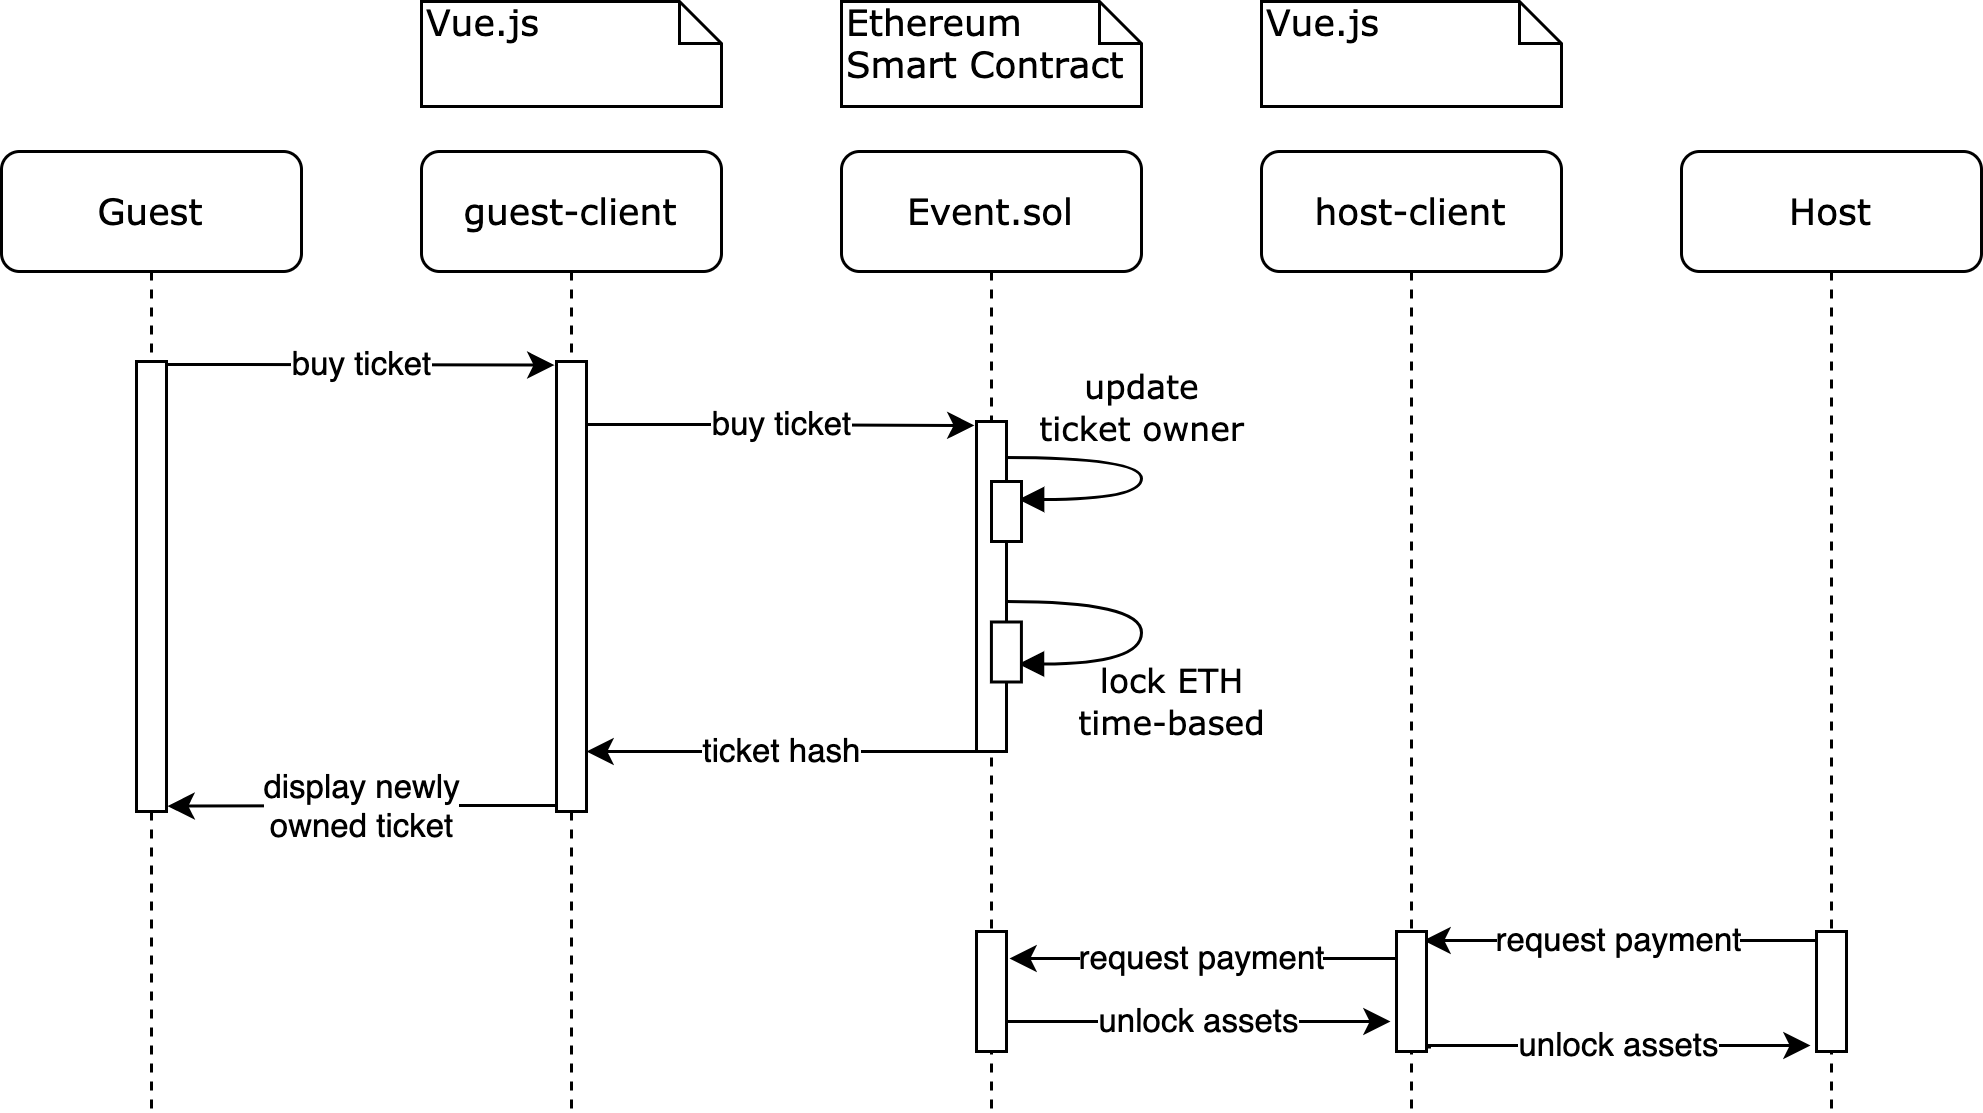
\includegraphics[width=16cm]{design/diagrams/BuyTicket.png}
    \caption{Ticket Sale Sequence Diagram}
    \label{fig:buyticket-sequence-diagram}
\end{figure}

\subsection{Presale}
The sequence diagram in Figure \ref{fig:presale-seuquence-diagram} illustrates how a guest can participate in a ticket presale. When registering for the presale, the ticket price is locked in the SC. The user has the option to opt-out at any time and get the locked ETH back. The event host decides when the presale ends. After this defined end time, the Event SC uses a source of randomness to determine the winners of the presale (see section\ref{section:imp:presale}). If a guest is part of the winners, he can mint his ticket. If not, the guest can claim the spent ETH back.

\begin{figure}[H]
    \centering
    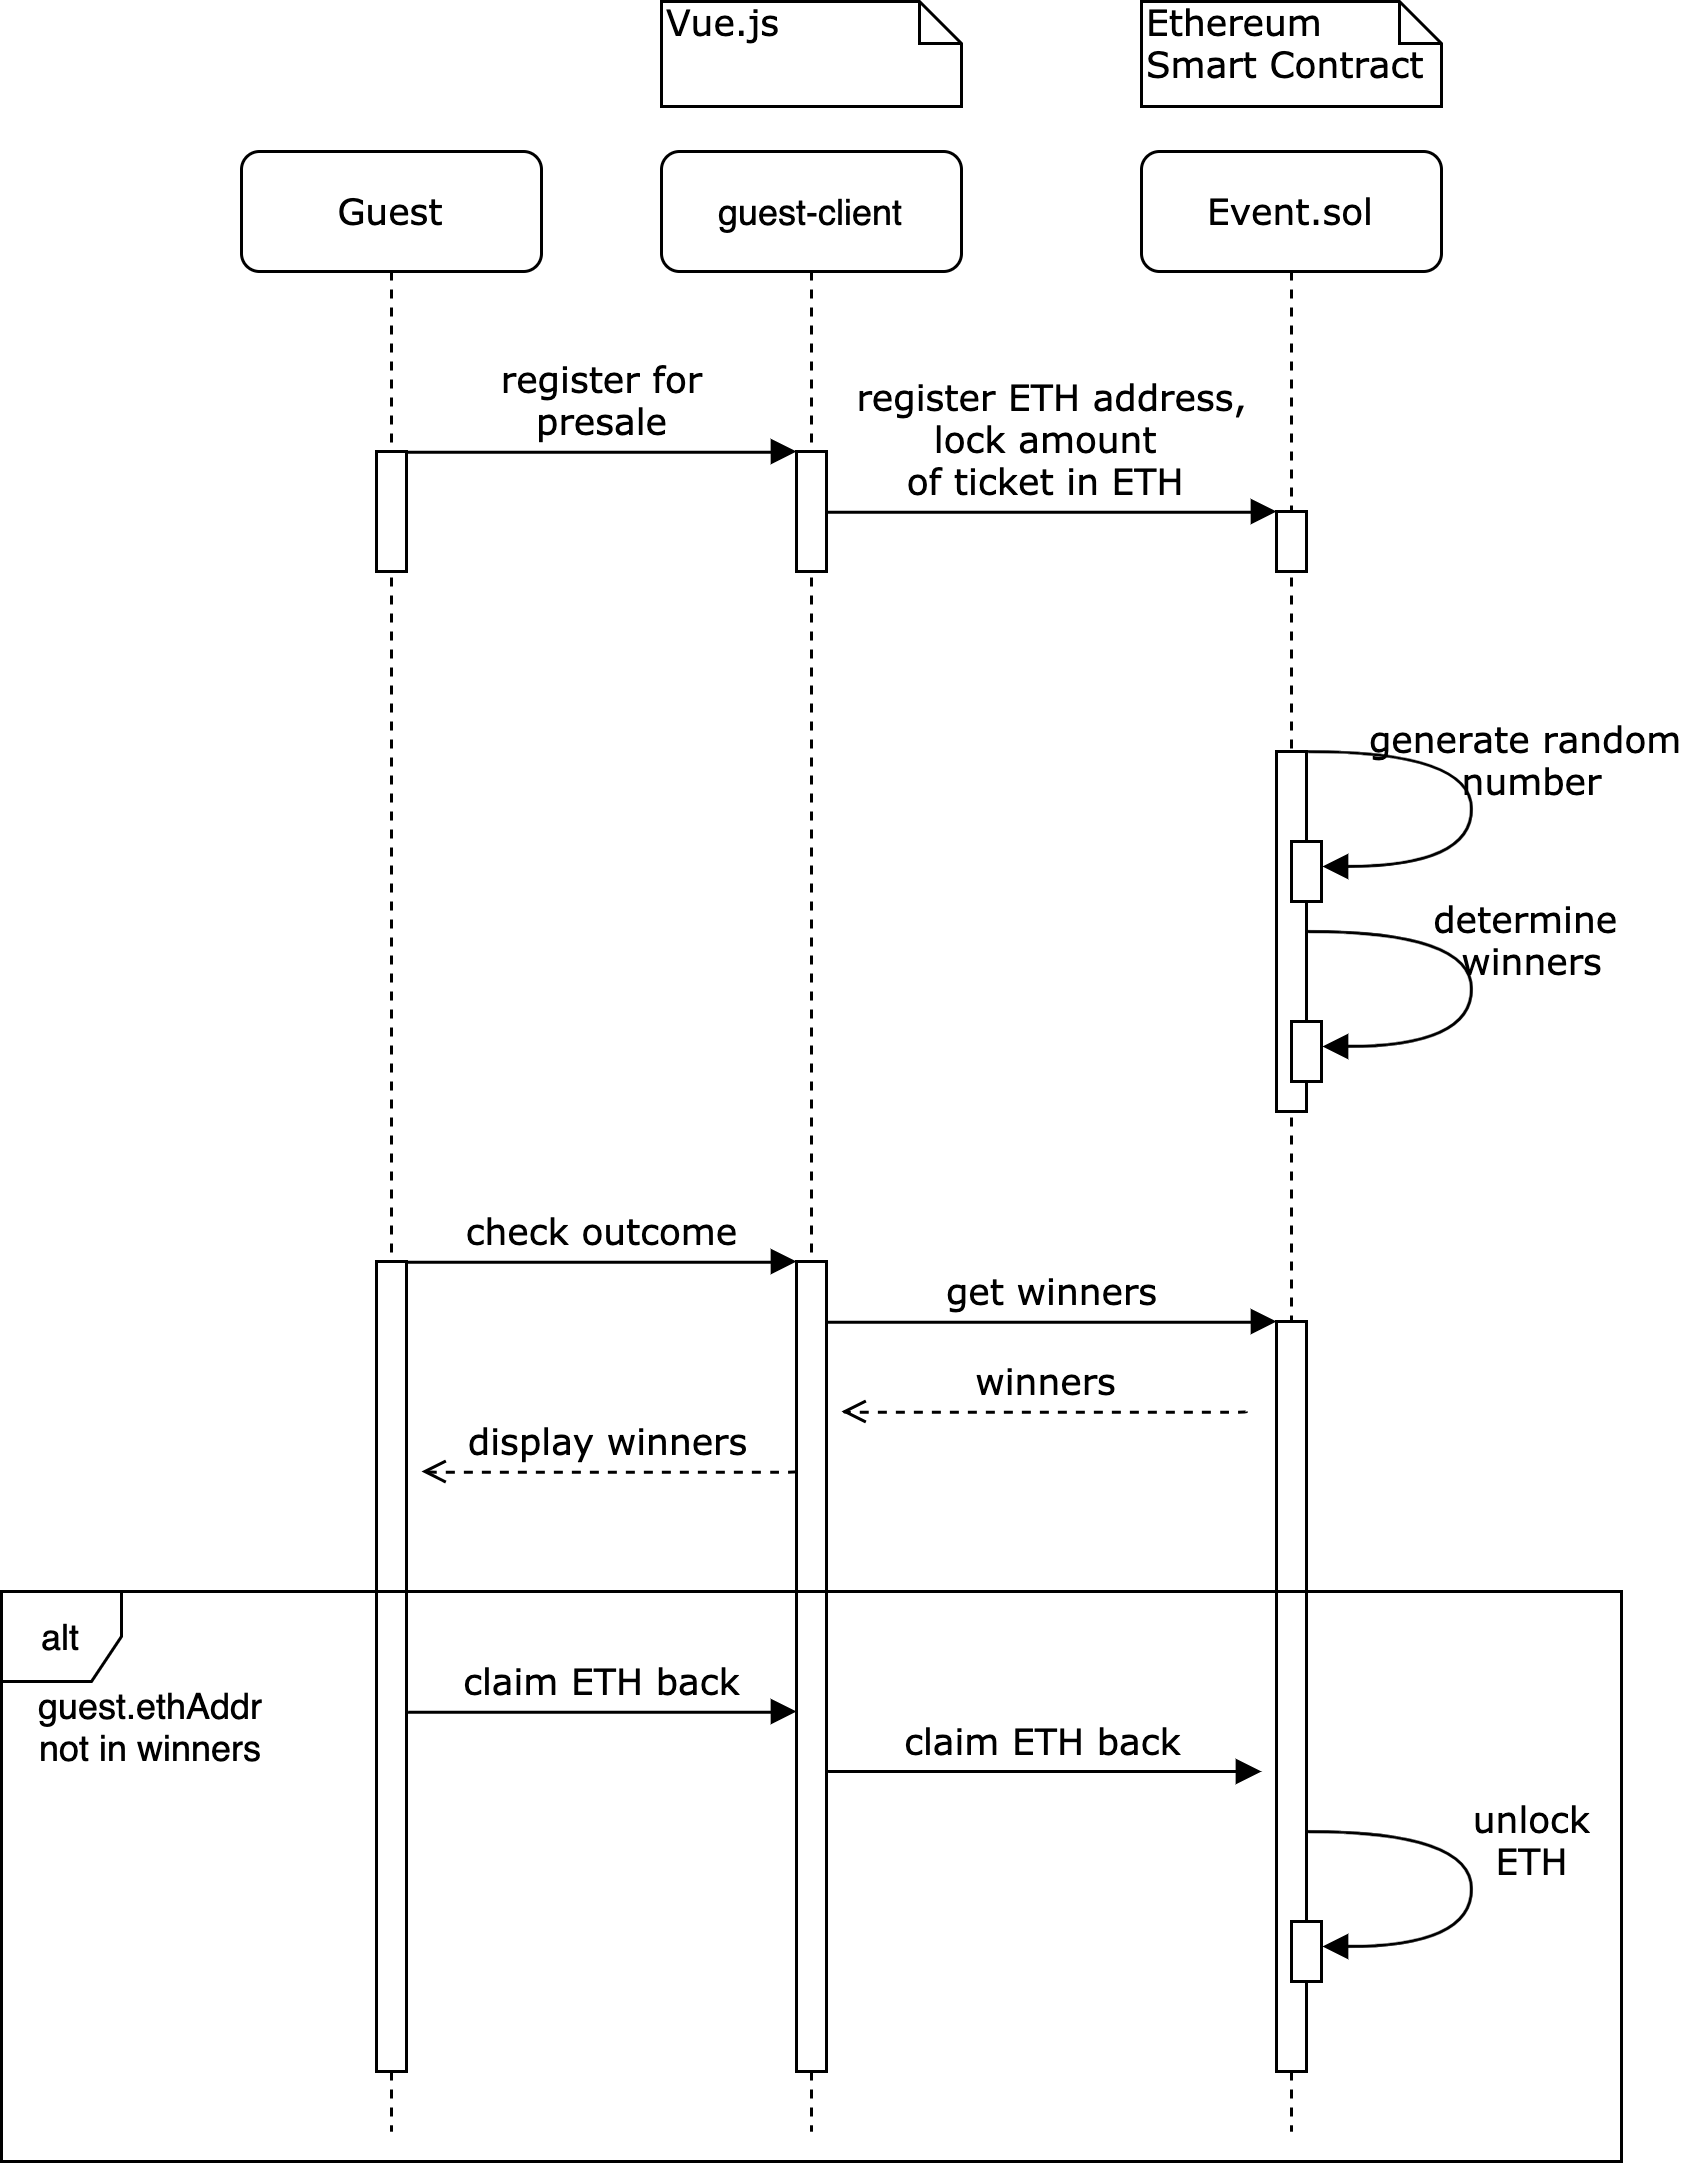
\includegraphics[width=14cm]{design/diagrams/presale.png}
    \caption{Presale Sequence Diagram}
    \label{fig:presale-seuquence-diagram}
\end{figure}

\subsection{Buy a Ticket from an Affiliate Link}
To broaden an event's visibility, a host may want to hire affiliates to promote their event. To do so, the host can register affiliates on the event SC, so that the affiliate can distribute a link containing his Ethereum address as query segment. The buying process is the same as in Figure \ref{fig:buyticket-sequence-diagram}. However, the affiliate's address is also forwarded to the SC and is linked to the bought ticket as well. After the event, when the ticket prices in ETH are unlocked, the affiliate can request to receive the award from each ticket that was sold holding his address as affiliate.
\begin{figure}[H]
    \centering
    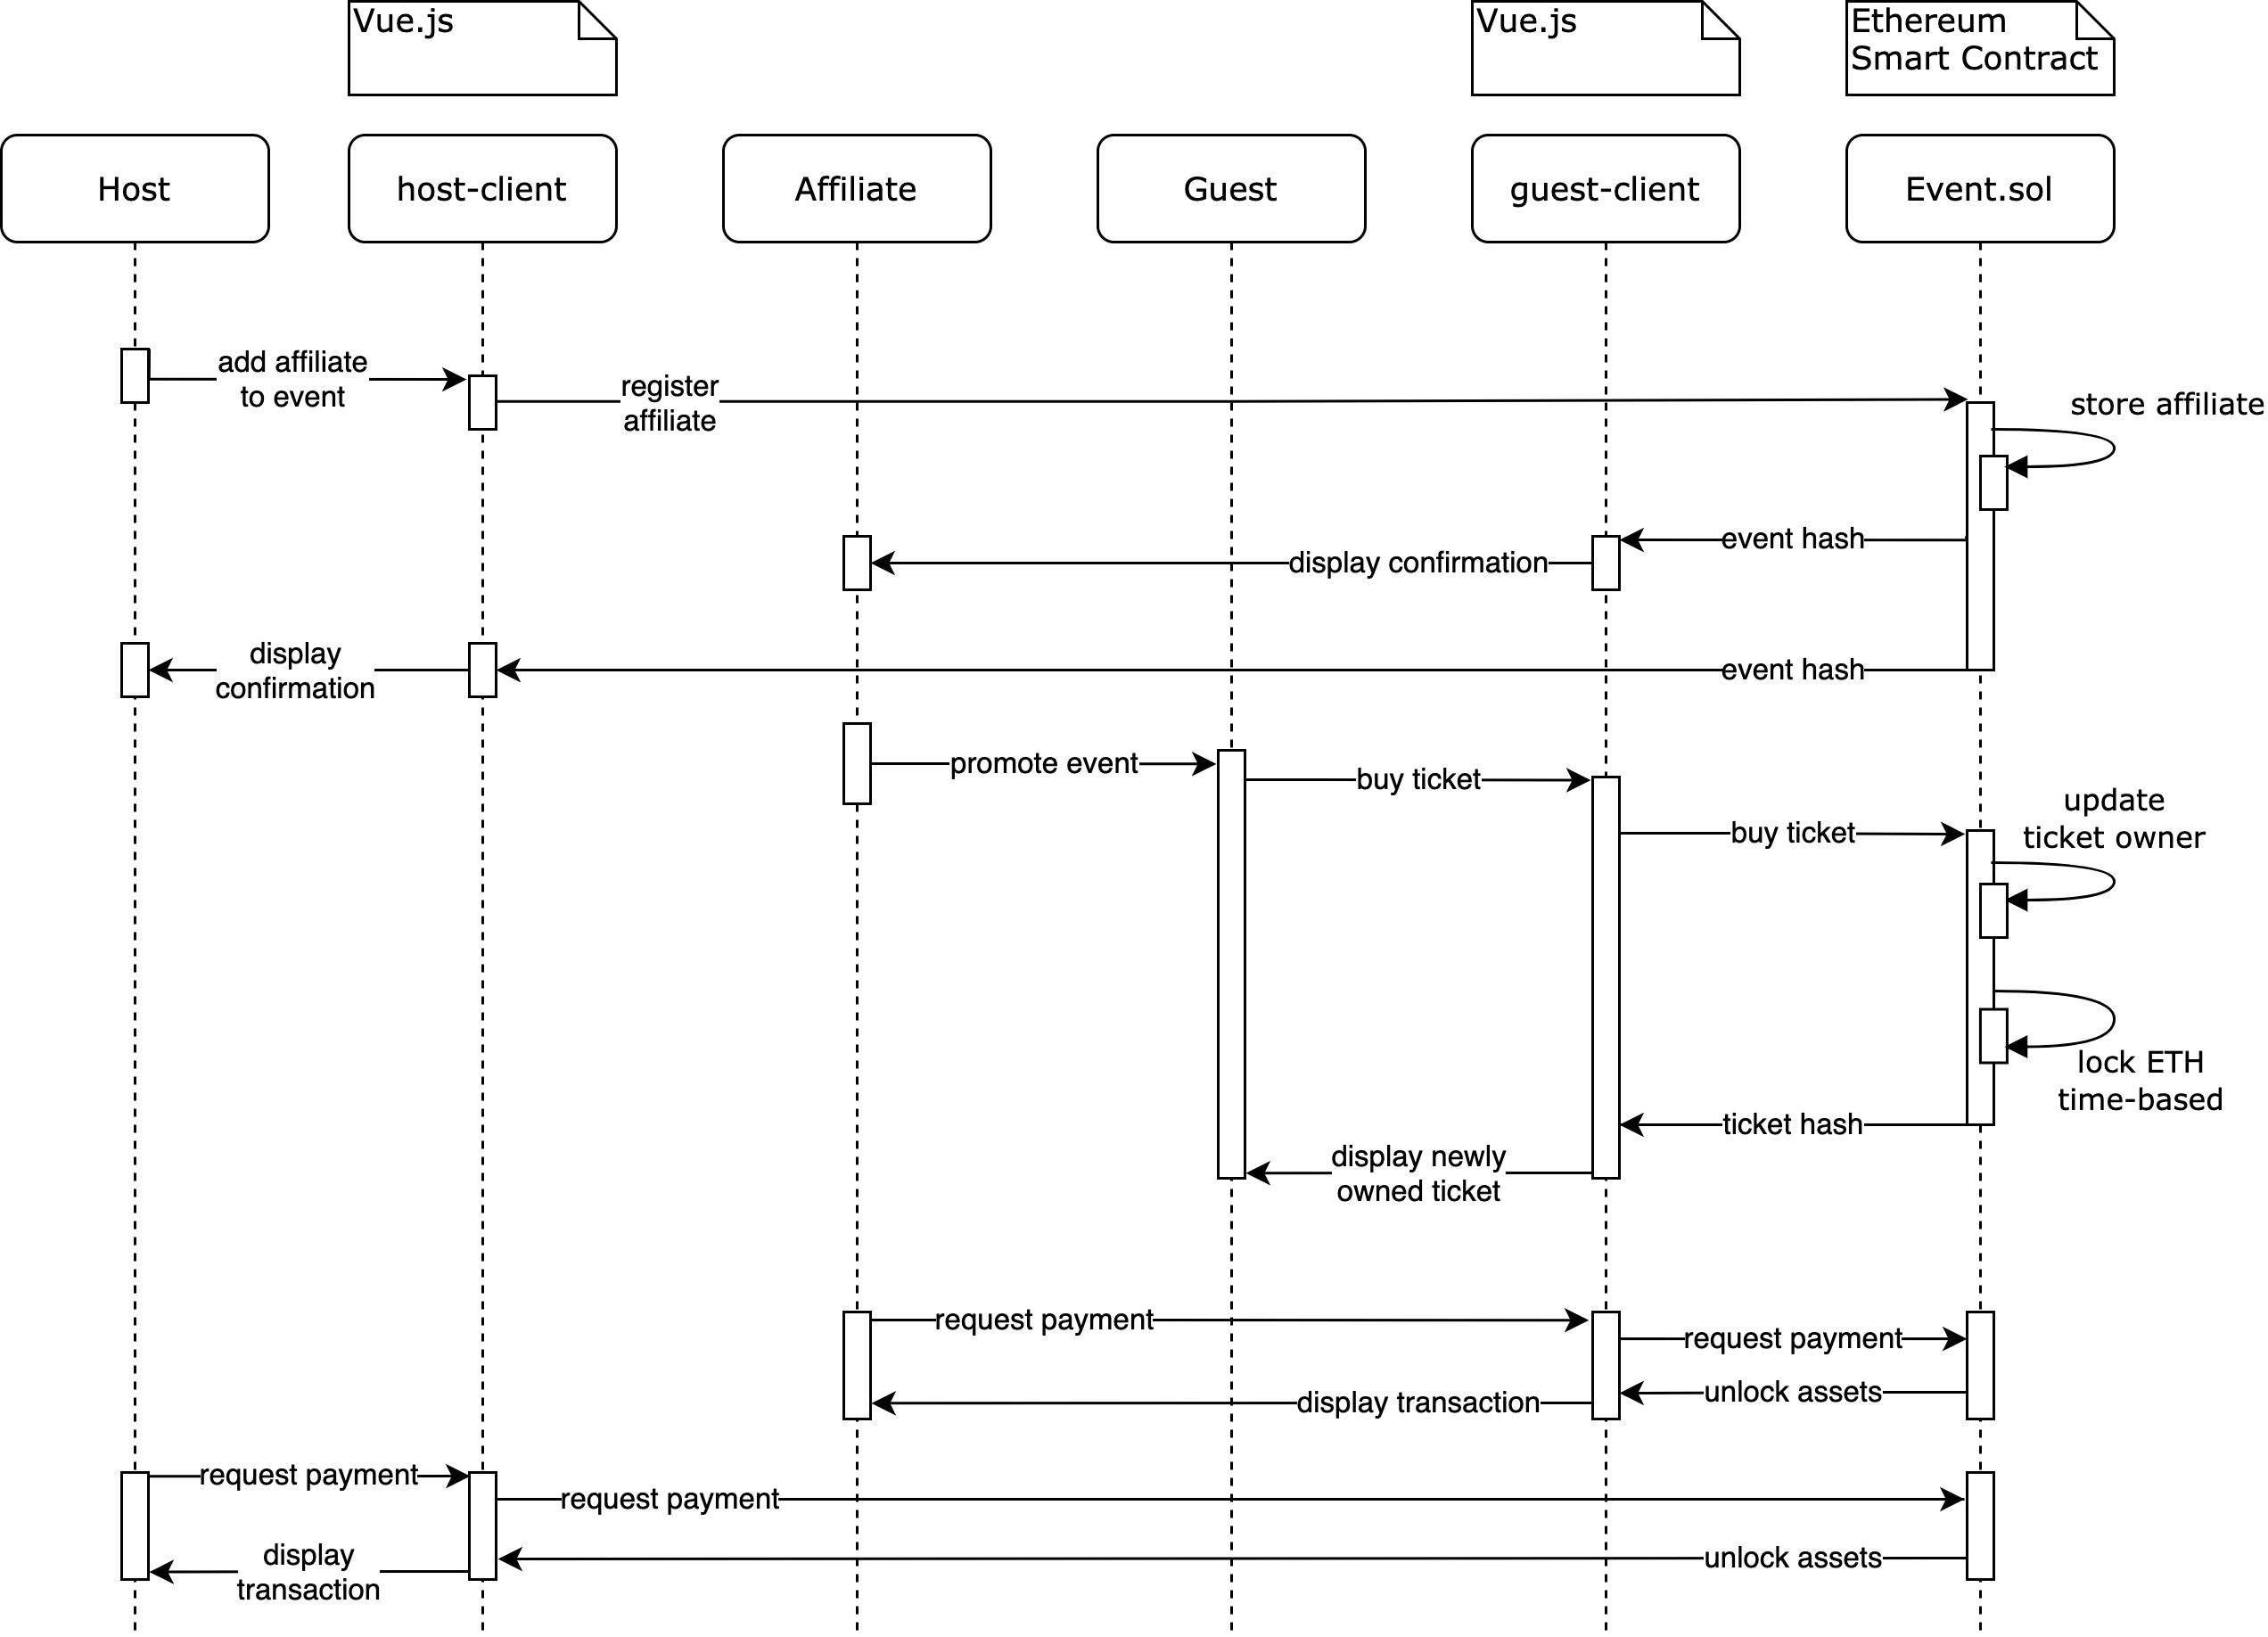
\includegraphics[width=16cm]{design/diagrams/BuyTicketFromAffiliateLink.png}
    \caption{Ticket Sale from Affiliate Link Sequence Diagram}
    \label{fig:buyticket-from-affiliate-diagram}
\end{figure}

\subsection{Identity Registration}
In Switzerland, to get a new phone number, you have to provide your passport details. Therefore a scalper cannot go through the process of approving his identity multiple times. The sequence diagram in Figure \ref{fig:identity-registration-airbnb} illustrates how a guest can prove his ownership of his phone number. To do so, the guest uses the \textit{guest-client} application to register an identity verification request. This request will be forwarded to the \textit{identity-approver} application. The identity approver is a trusted entity that checks if a user is in control of a certain Ethereum address, phone number, etc. In this scenario the user proofs his ownership of a phone number.  The idea of the identity approver is to store the uniqueness characteristic of that phone number and link it to a Ethereum address without the need of creating another KYC process. 

The identity approver generates a random sequence and sends it back to the identity the guest wants to proof ownership of. The guest receives the random sequence and enters it into the guest-client. The guest is then asked to sign the random sequence using his Ethereum address. The \textit{identity-approver} checks the signature for its validity. If this check completes successfully, a proof is generated.

Important to note is that the \textit{identity-approver} is a trusted entity. However, the goal is to build an application that does not rely on a single trusted entity. Thus, a system is envisioned where an event host can select from different identity approver and providers. It should even be possible that an event host can also act as the identity provider and approver. This would make sense for a large event company that want to make sure that no fraud is made by third parties. 

\begin{figure}[H]
    \centering
    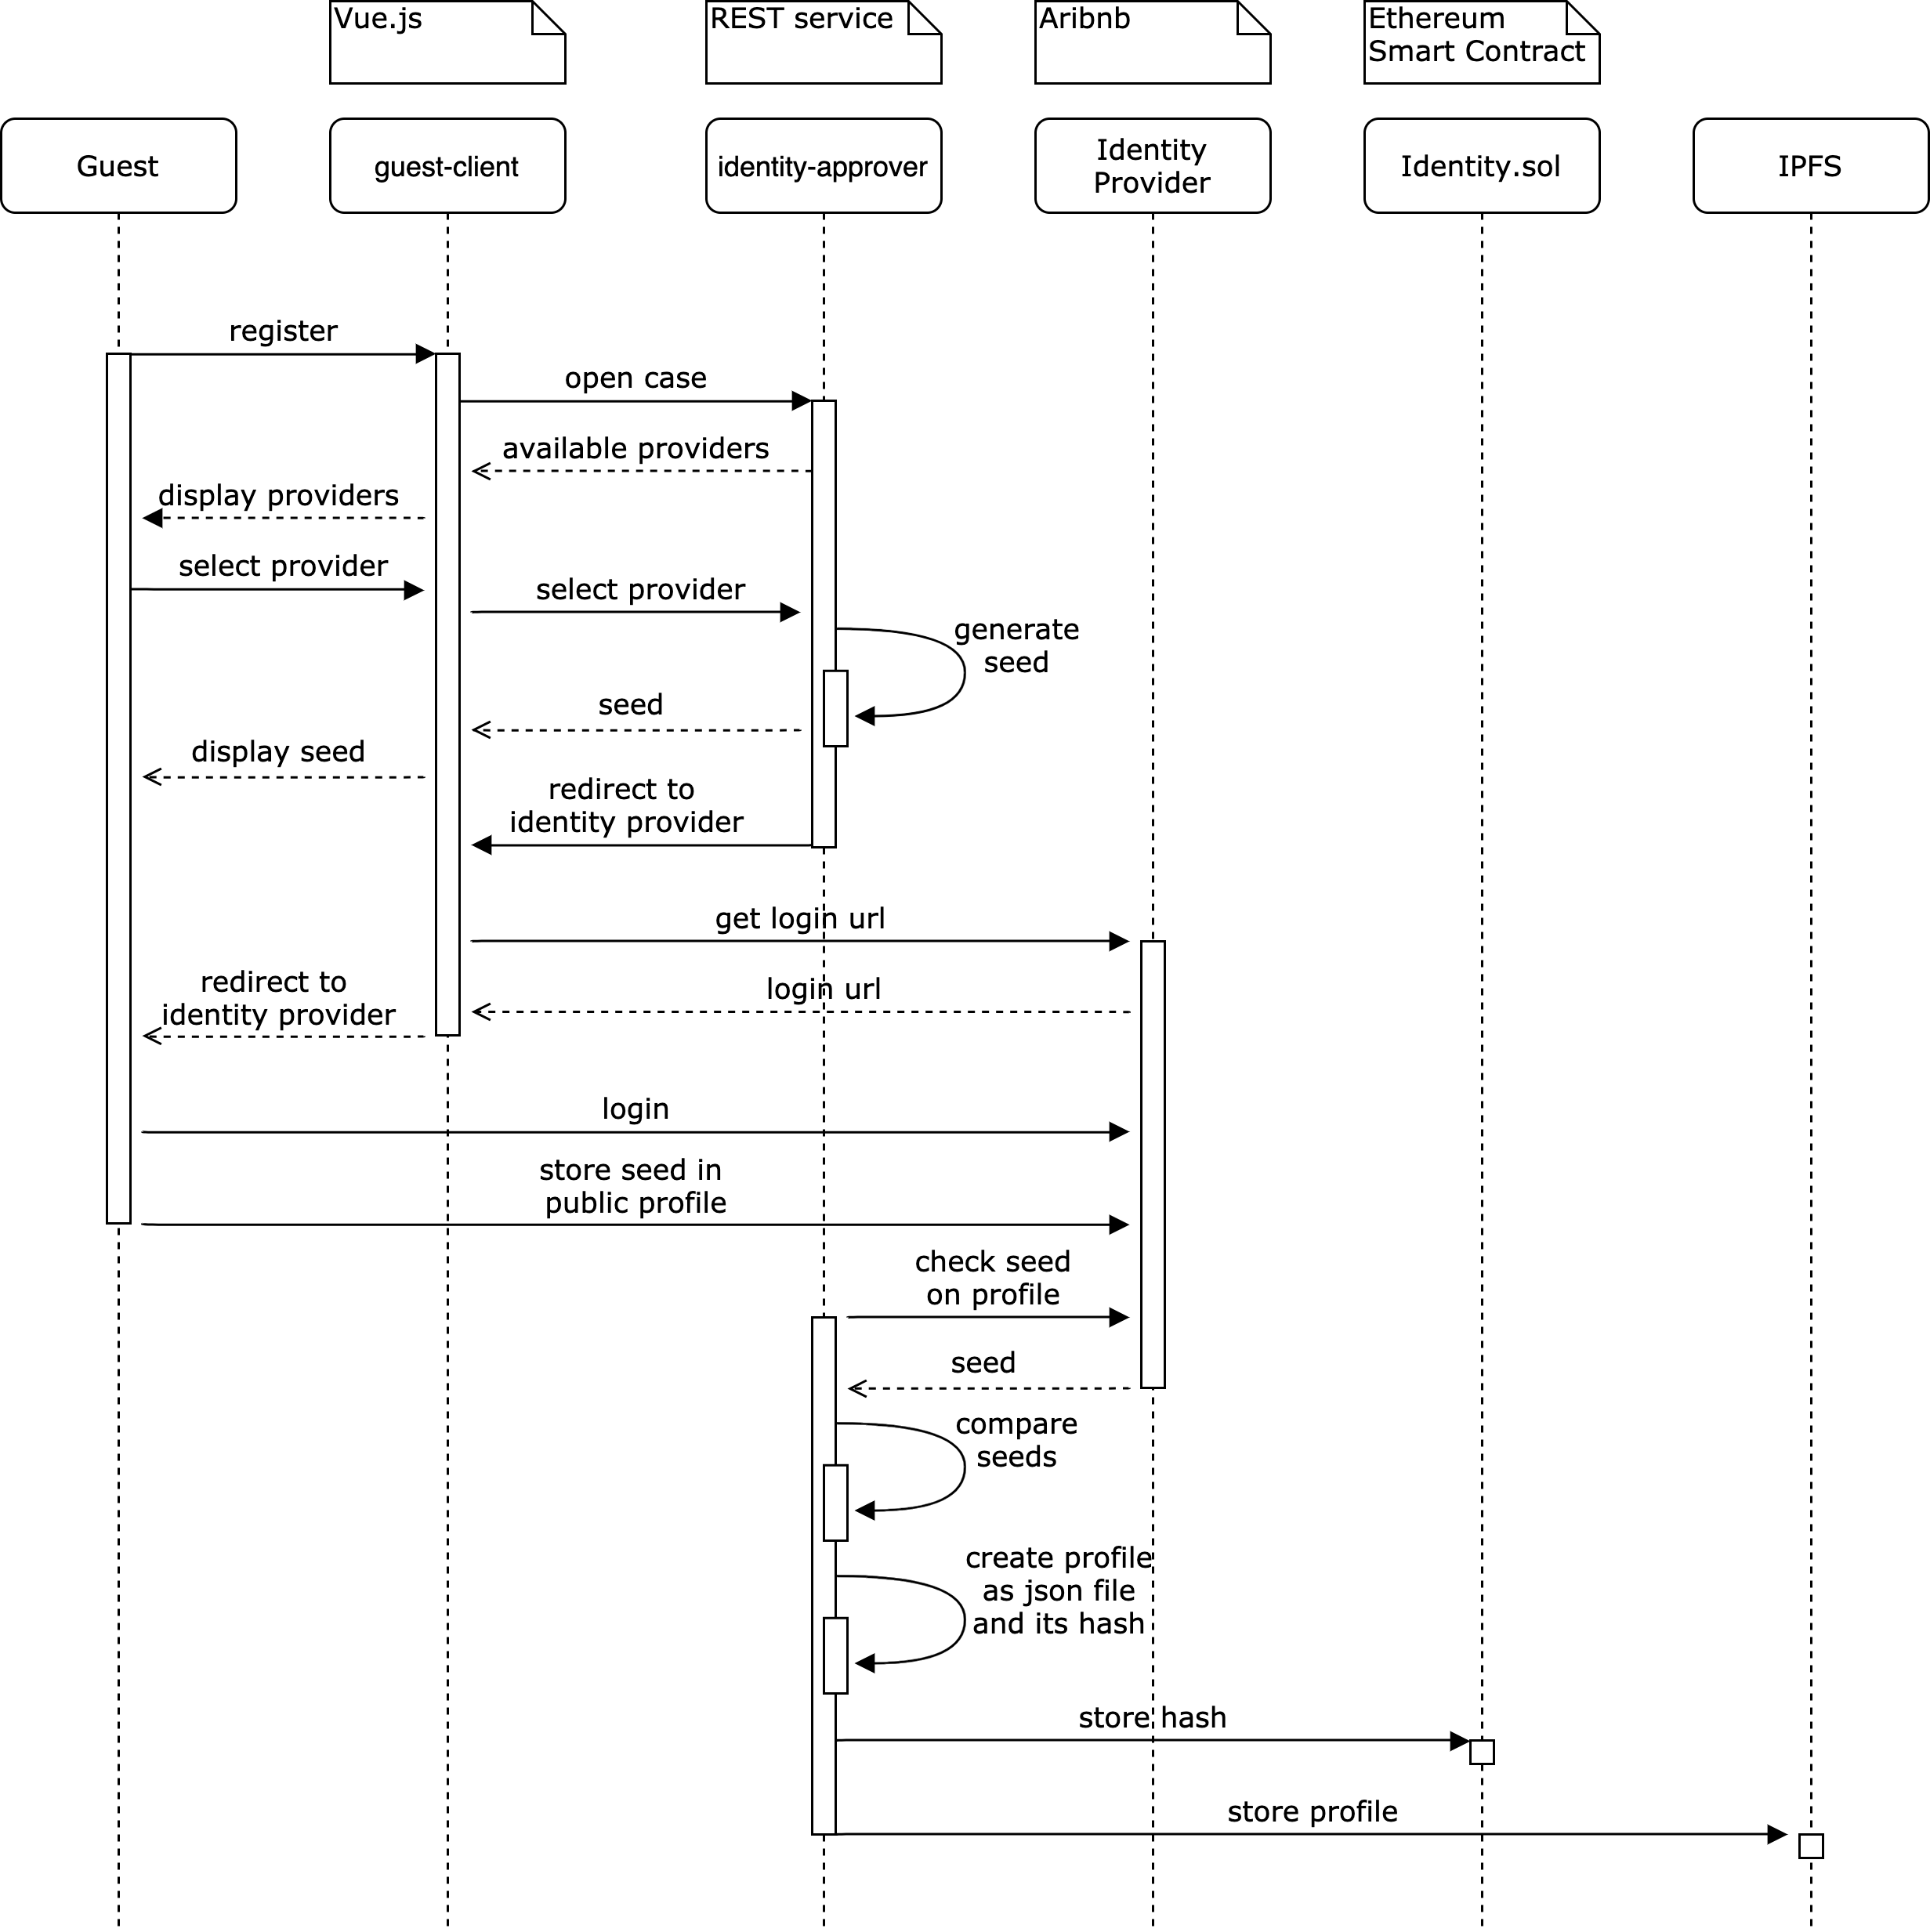
\includegraphics[width=16cm]{design/diagrams/identy-registration-airbnb.png}
    \caption{Identity Registration Phone number}
    \label{fig:identity-registration-airbnb}
\end{figure}

\subsection{Resell Ticket}
The guest logs into his account. The guest-client the gets all the Tickets owned by the guest, that are still valid. It then retrieves the ticket metadata form the IPFS storage. After the metadata has been retrieved, the guest gets shown the ticked owned by him. the guest then chooses the ticket he does no longer want to have and therefore selects the option to sell his ticket in the guest-client. This lists the ticket on the aftermarket. Whenever the ticket is bought by another guest, the money used to buy the ticket is directly transferred to the wallet of the seller of the ticket. When the guest checks his balance again, he will see the added funds.

This process is illustrated in the following sequence diagram.

\begin{figure}[H]
    \centering
    \includegraphics[width=16cm]{design/diagrams/Resell Ticket.png}
    \caption{Resell ticket}
    \label{fig:Resell-ticket}
\end{figure}

 


\subsection{Buy Ticket From Reseller}
\begin{figure}[H]
    \centering
    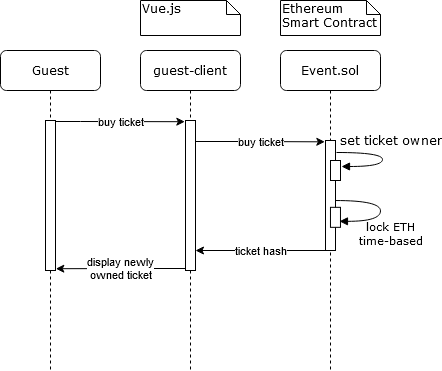
\includegraphics[width=12cm]{design/diagrams/BuyTicketFromResell.png}
    \caption{Buy Ticker from reseller}
    \label{fig:buyFromResell}
\end{figure}
The process of buying a ticket from the resell market looks exactly the same as buying directly from the host directly from the customers point-of-view, as depicted in \ref{fig:buyFromResell}. The Guest first connects to his wallet through his private key on the guest web application. Then he selects the event he is interested in and chooses to buy a ticket, which invokes the corresponding SC. Exactly as seen in \ref{fig:buyticket-sequence-diagram}, the SC locks the price of the ticket until the event has passed and returns the ticket hash to the guest web application, where it is displayed to the guest.

\subsection{Access Control}\label{subsection:access-control}

\begin{figure}[H]
    \centering
    \includegraphics[width=16cm]{design/diagrams/AcessControl.png}
    \caption{Access Control Sequence Diagram}
    \label{fig:access-controll}
\end{figure}

As the guest wants to gain access to the event, he is confronted with the entrance control. As the ticket is linked to the Ethereum address of the guest, he just has to prove the ownership of the given Ethereum address. In order to do this, the guest has to provide a signature of a message. This signature together with the message and the guest's public address can then be verified which ultimately proves that the guest owns this Ethereum address.

For this process three components are necessary. First of all, access terminal web applications (see section \ref{design:access-terminal}) are intended to run on tablet at the venue. They are used to display messages to be signed, a backend is needed to handle the signatures and keeping track of the state of the terminals and an embedded camera feature in the guest client application is required to scan the information from the terminal, sign the message and sending the signature to the backend for verification.

%Access terminals are placed at the respective entrances to display messages to be signed. A backend spring application provides an API to register terminals, create new messages for signing, verify signatures and check whether a ticket of the guest actually exists and was not already used to enter the event. 

%Access Terminals (see Subsection \ref{design:access-terminal}) are placed at the respective entrances. These terminals have to be registered with a secret code stored in the backend. When a terminal is registered, it is allocated a unique random sequence, which is stored in the backend and in the terminal application.

The entrance control terminals (see Subsection \ref{design:access-terminal}) are registered at the backend. Every terminal gets its unique identifier. The terminal then requests a unique random sequence, which is stored with the corresponding terminal id in the backend. This random sequence is then displayed alongside the backend URL as a QR-code on the terminal. The guest reads the QR-Code and extracts the random sequence. He then proceeds to sign the sequence using his Ethereum address proofing his ownership. The signature, the Ethereum address, the number of tickets he wants to use and the random sequence are then sent to the backend. The backend then evaluates the validity of the signature. After that, it is checked, whether the random sequence exists and the block chain is queried, to check, whether the Ethereum address actually holds enough tickets. It is also checked, whether this ticket already entered the venue. When all these checks are successful, the terminal, specified by its id, is messaged to let the guest pass. At the same time, the Ethereum address and the corresponding ticket are added to the database, that tracks the area the ticket owner are in. This implementation also holds for changing from different areas in a venue, for example accessing the VIP are from the general area of the venue.


%\begin{figure}[H]
%    \centering
%    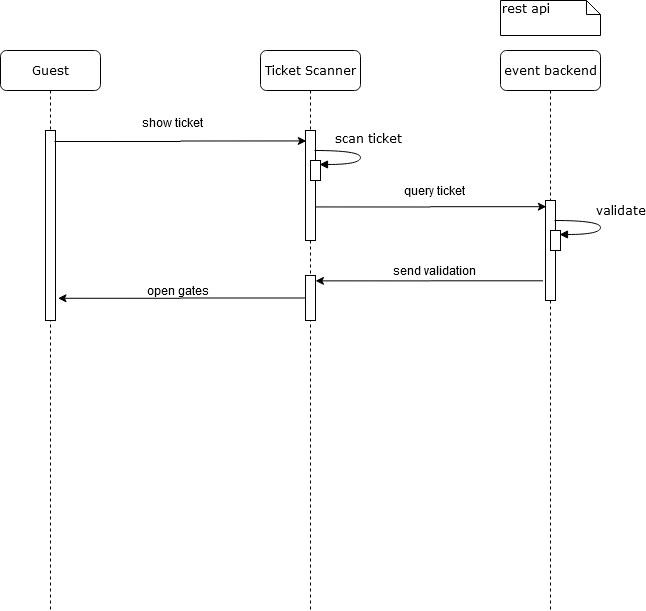
\includegraphics[width=14cm]{design/diagrams/entrance.png}
%    \caption{Entrance Control}
%    \label{fig:entranceControl}
%\end{figure}

%The sequence diagram in \ref{fig:entranceControl} depicts the process applied at the event gates for handling entrance control. The guest presents his ticket to the employee at the gate in form of a QR-code on his phone. The employee scans the code using the ticket scanner mobile application, which invokes a call to the rest API on the event backend, which contains a database with all tickets and the public keys of their respective owners. Once the Ticket Scanner application receives the confirmation from the server that the code is valid, the guest is granted access to the event.



% \subsection{Event Cancellation}
%This Section demonstrates how a guest can issue a report if an event was fraudulent or did not take place and the event host did not pay back the ticket price. 

%The sequence diagram in Figure \ref{fig:dispute-resolution-approved} shows how a guest rightfully reports a dispute and in Figure \ref{fig:dispute-resolution-rejected} the guest is not entitled to issue a dispute. 

%When the host creates an event, a fixed amount of ETH is locked as a deposit as well as a trusted third party is used to verify the guest's identification as explained in Figure \ref{fig:identity-registration-airbnb}. This party also acts as a dispute resolver. It is envisioned that this entity consists of multiple parties but for simplicity reasons it is shown as one ETH account. The deposit is locked until the challenge period is over. During the challenge period a guest can report fraudulent events.

%When the dispute resolver receives examination requests, they contact the event host for access proof. These proofs can only be generated by the ticket holders and contain the event id and the date of access. If the host can provide such requests, the tickets were used to enter the venue. The claim that the event was fraudulent is wrong and the host deposit will be unlocked for the host when the challenge period is over. 


%\begin{figure}[H]
%    \centering
%    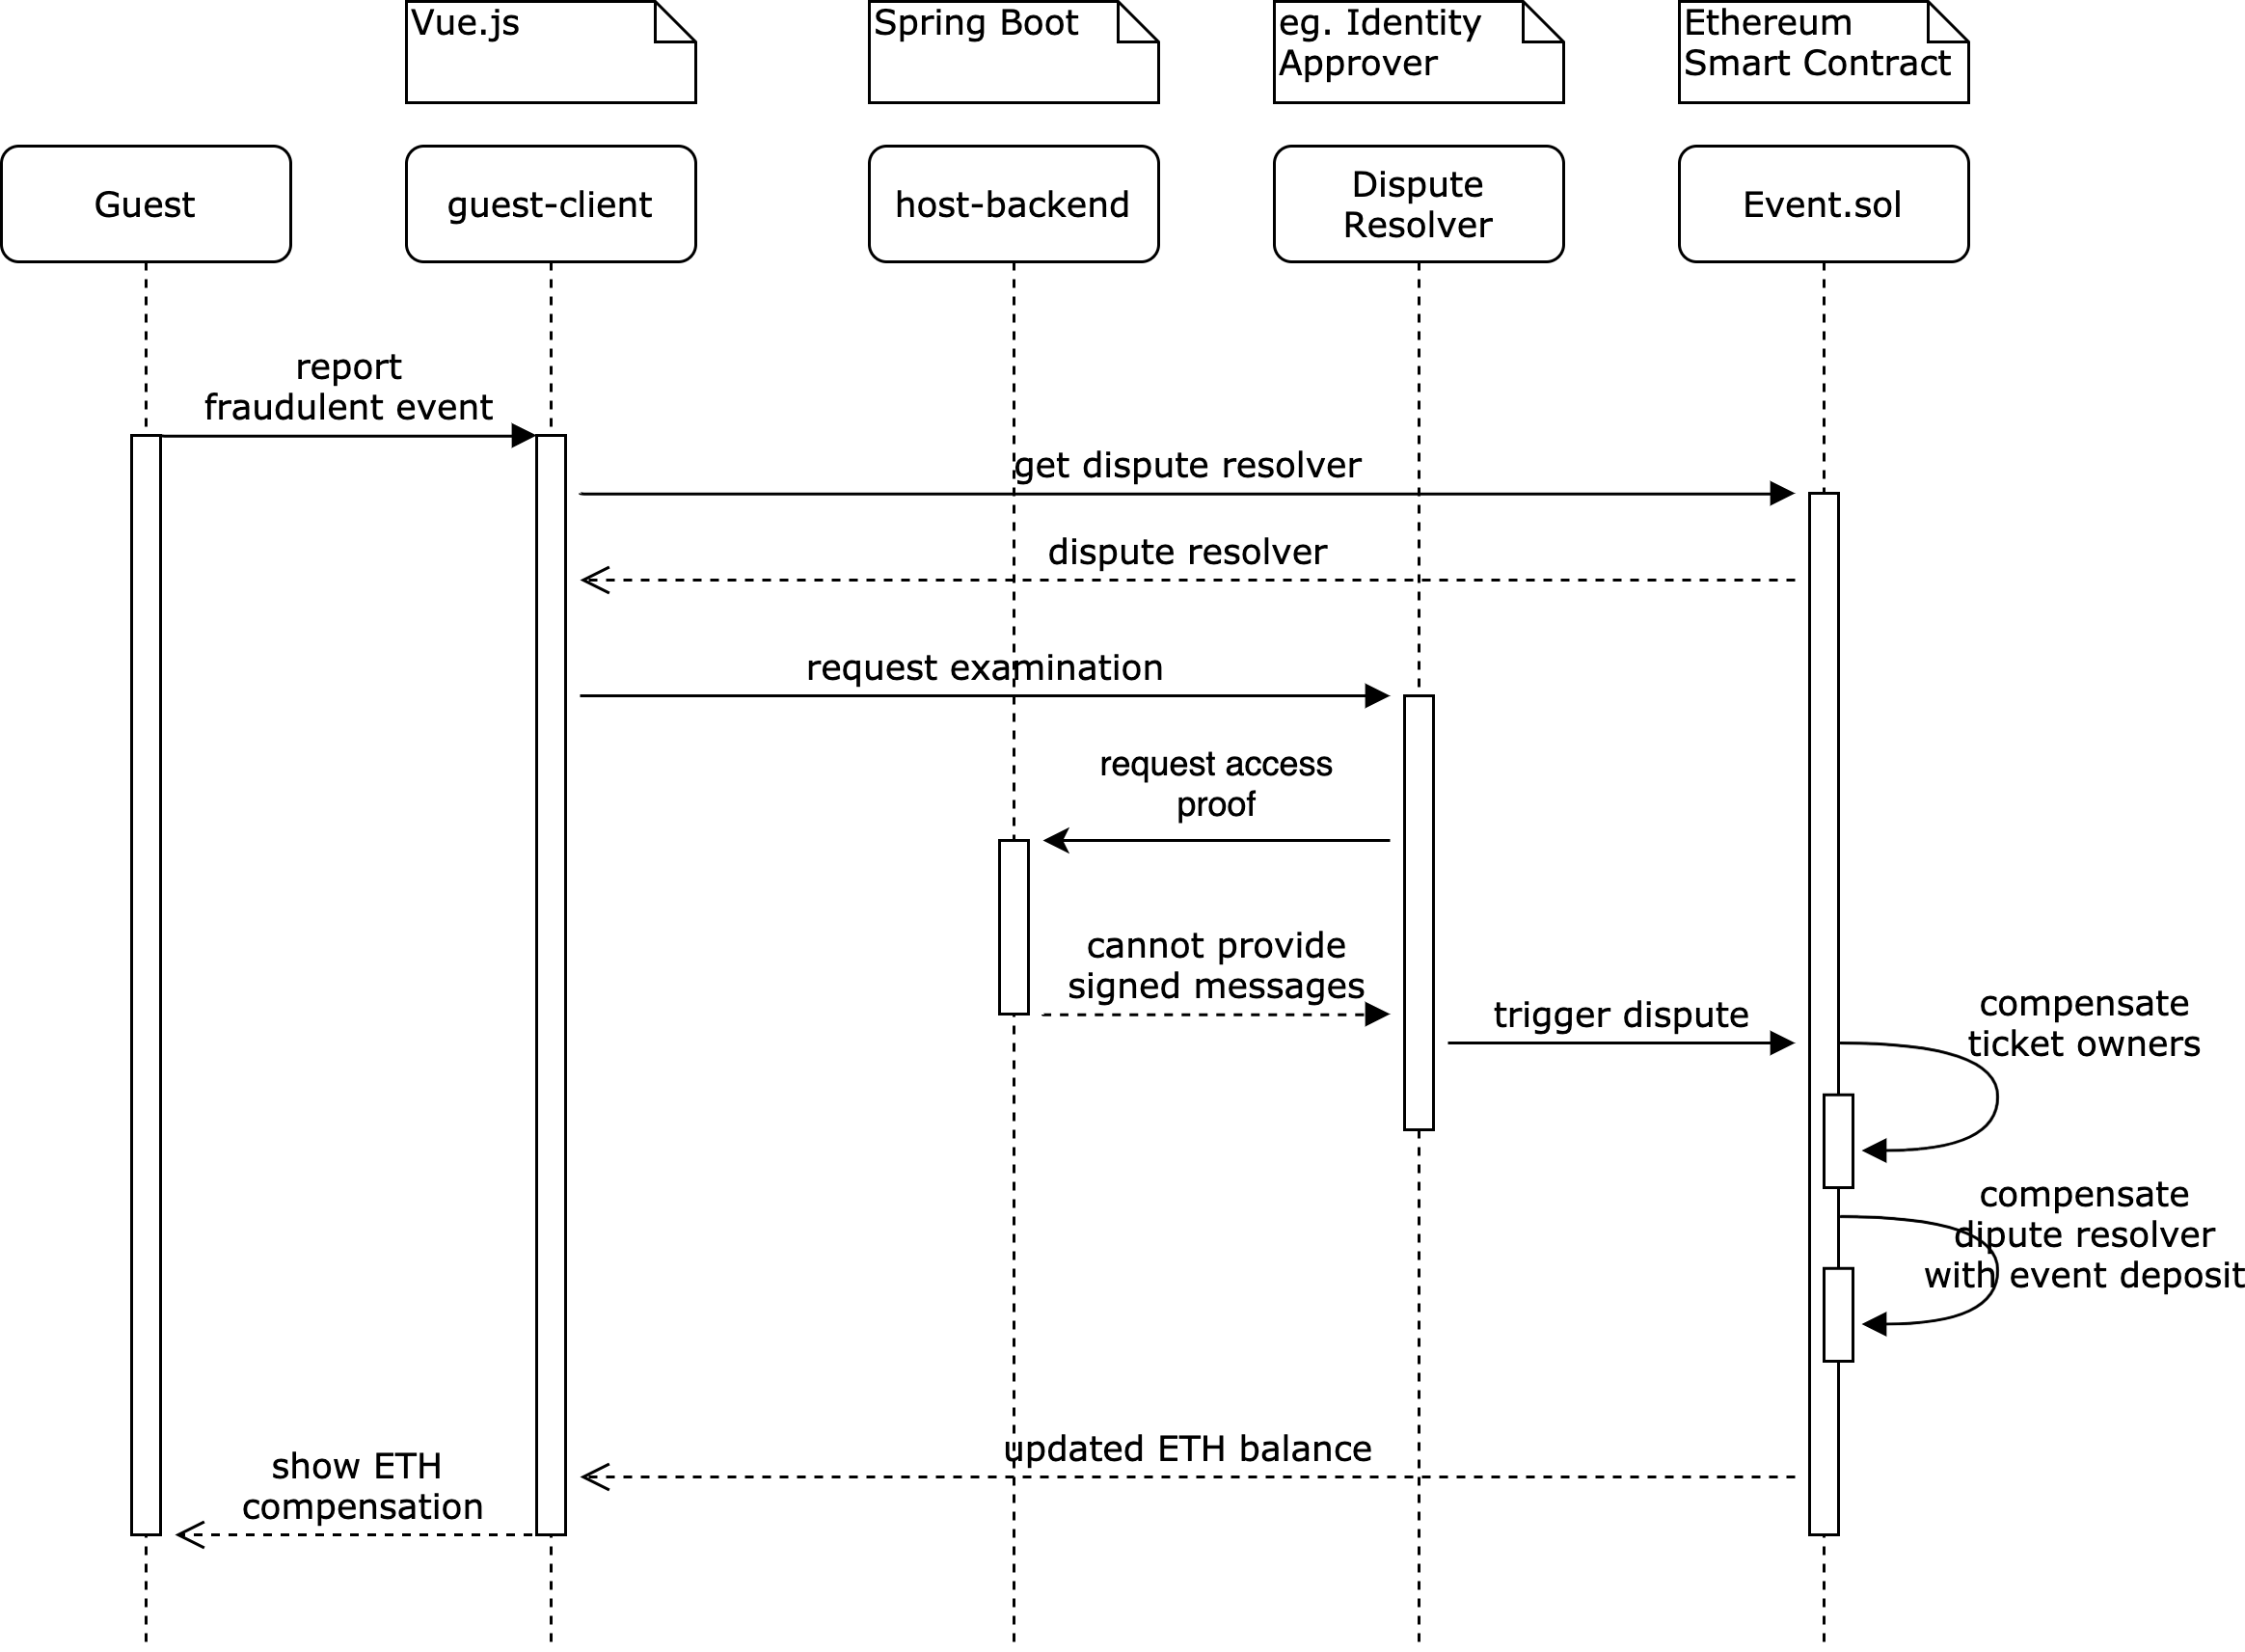
\includegraphics[width=16cm]{design/diagrams/dispute-resolution-approved.png}
%    \caption{Event Cancellation Approved}
%    \label{fig:dispute-resolution-approved}
%\end{figure}


%In the case where the event is fraudulent, the event host cannot provide signed proofs that tickets were used to enter the venue. The dispute resolver then calls the SC to send the locked ETH in the SC back to the ticket owners. Also the dispute resolver is compensated with the deposit that the event host initially had to deposit when the event was created. 

%\begin{figure}[H]
%    \centering
%    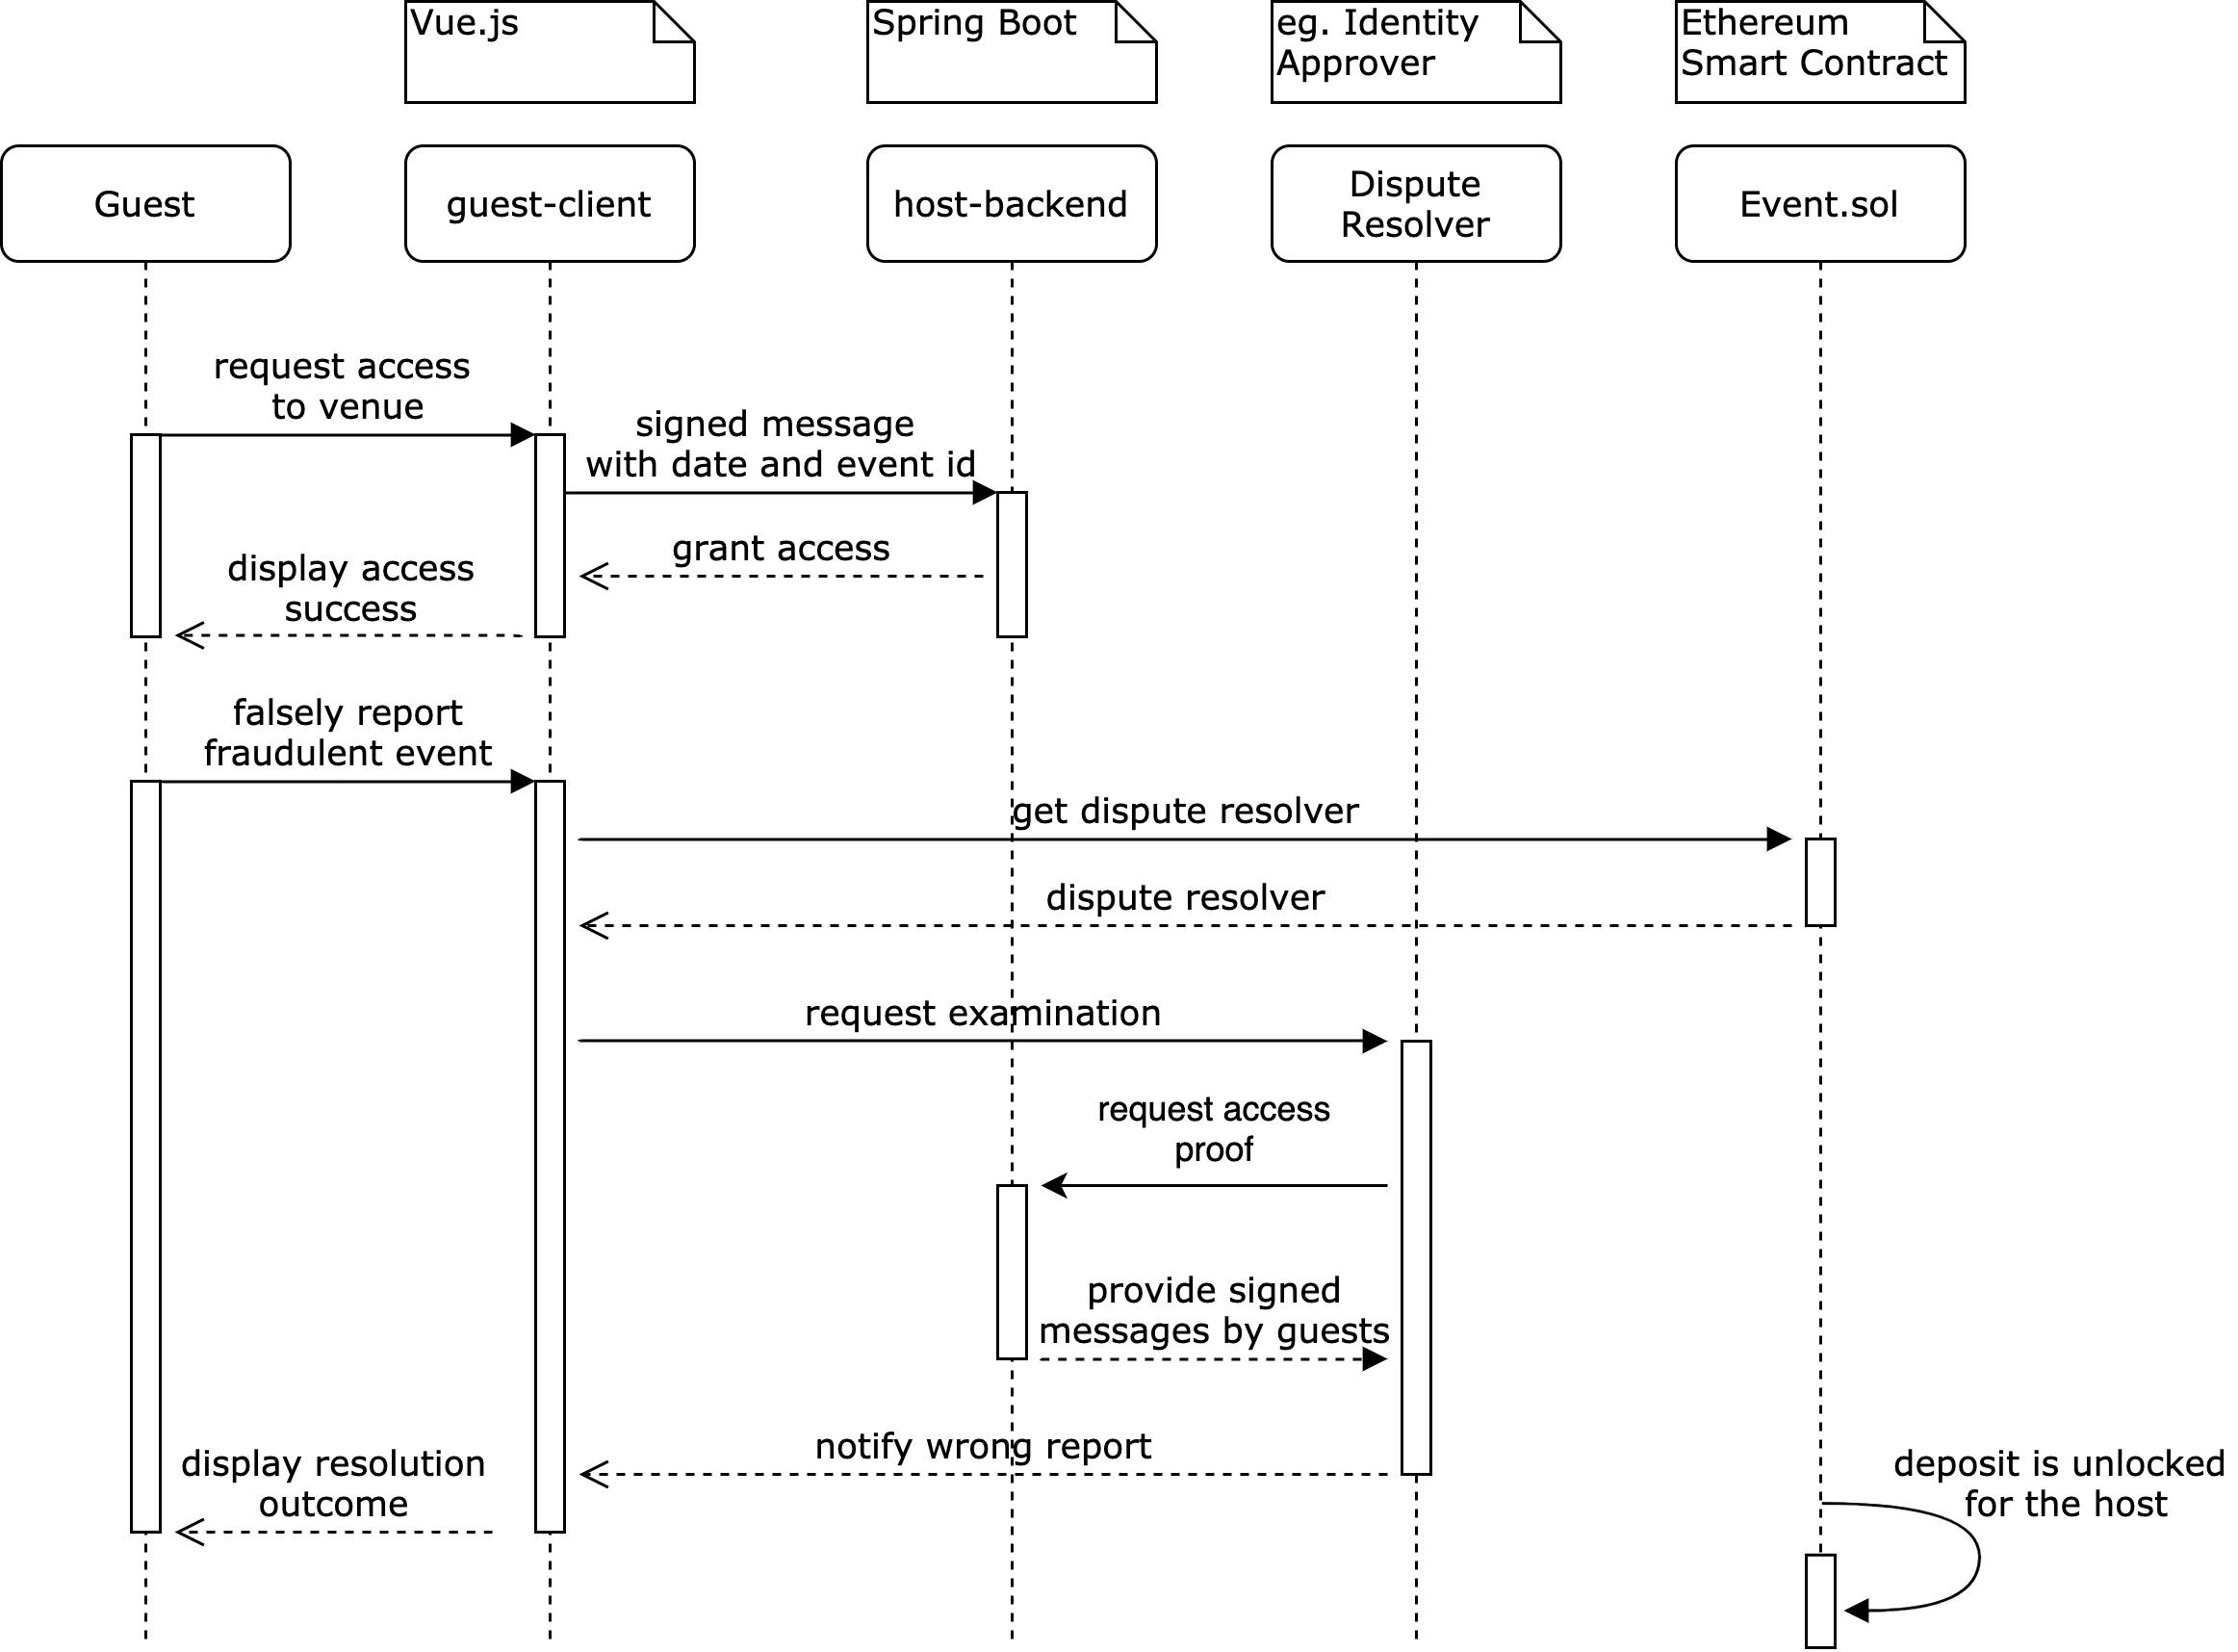
\includegraphics[width=16cm]{design/diagrams/dispute-resolution-rejected.png}
%    \caption{Event Cancellation Rejected}
%    \label{fig:dispute-resolution-rejected}
%\end{figure}
\section{Data Model}


\subsection{Smart Contract for Event Hosting}
The class diagram in Figure \ref{fig:event-data-model} illustrates how events are created and registered, tickets can be issued and distributed. Important to point out is that a presale only makes sense for fungible tickets. 
\begin{figure}[H]
    \centering
    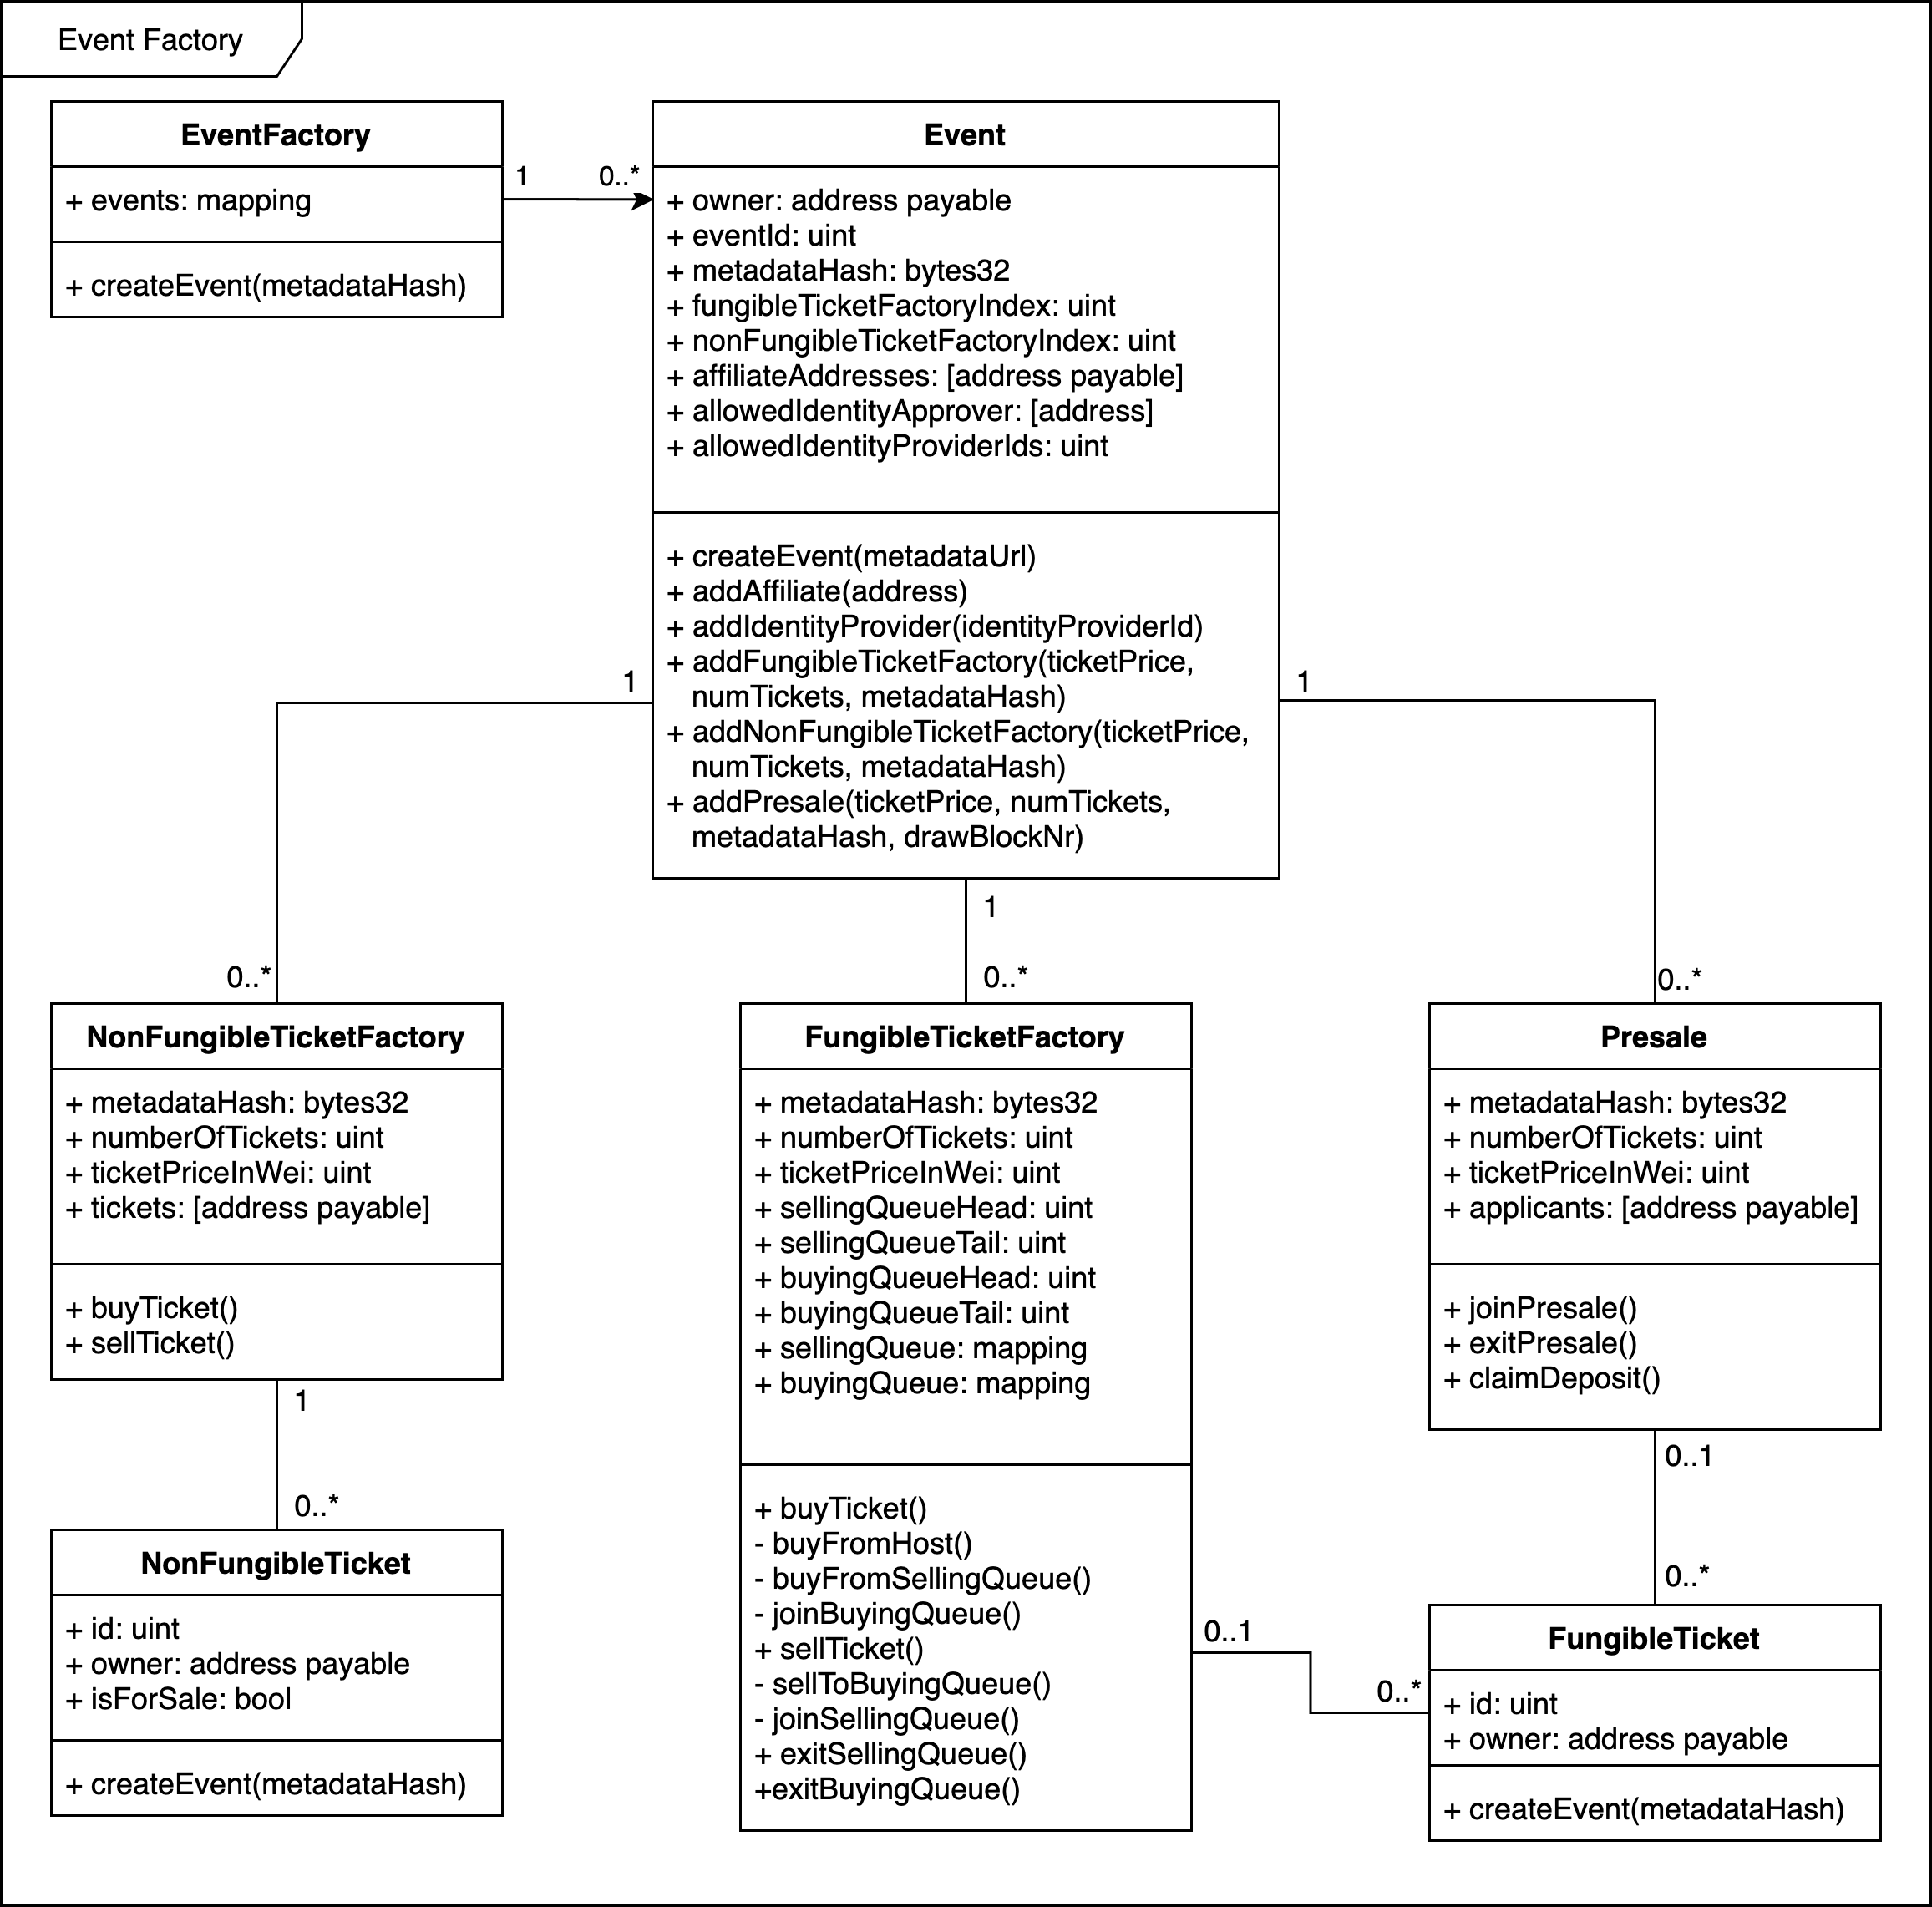
\includegraphics[width=16cm]{design/diagrams/event-factory-class-diagramm.png}
    \caption{Event Data Model}
    \label{fig:event-data-model}
\end{figure}

\subsection{Smart Contract for Identity Registration}

\subsection{RESTful Service for Identity Registration and Approval}
To interact with the identity approver, a Rest API as in Table \ref{tab:Identity-Reg-Rest-API} is used. The first step is to register an identity for approval. A secret will then be sent to this identity. In the next step, the identity is validated using the ETHadress and the secret received.

\begin{table}[H]
\caption{Identity Registration and Approval Rest API}
\label{tab:Identity-Reg-Rest-API}

\begin{tabular} { | m{0.3\textwidth} |m{0.1\textwidth}|m{0.2\textwidth}|m{0.2\textwidth} | }
\hline
Mapping & Type & Parameters & Return \\
\hline
  /addEmailIdentity & Post & eMail & boolean \\ 
\hline
/validateEmailIdentity & Post & eMail  & EmailIdentity \\ 
& &secret  & \\
& & signedSecret  & \\
& & ethAddress & \\
\hline
/addPhoneIdentity   & Post & phoneNr & boolean \\ 
\hline
/validatePhoneIdentity & Post & phoneNr & PhoneIdentity \\ 
& &secret  & \\
& & signedSecret  & \\
& & ethAddress & \\
\hline
\end{tabular}

\end{table}


\subsection{RESTful Service for Access Control}

\section{Technology Stack}\label{chapter:technology}

This section covers the technologies used within all separate parts of the ticketing platform.

\subsection{Client Web Applications}

The guest-client web application is the GUI provided for potential event guests interested in buying or selling tickets. The host-client web application is a tool for event organizers, which allows them to create events on the platform as well as to manage their events including the tickets.

Both web applications are built with Vue.js, a client-side JavaScript framework. Vue.js allows to integrate reactivity and application state management into websites and convinces through natively available modules for most essential parts of a modern web application.

In order to interact with the BC, the web3.js library is used. Web3.js provides wrapper functionality for data fetching from the BC and invoking remote SC calls. 
As mentioned in \ref{section:data-model}, the storage capabilities of SCs are highly limited. Thus, all event-related information (metadata) which is not critical for the core logic of the platform is stored externally. To keep the architecture as decentralized as possible, the metadata is stored on Inter Planetary File System (IPFS). IPFS is a peer-to-peer distributed file system, which is accessed from the guest-client application through a JavaScript API. To reduce the amount of remote calls to the BC and IPFS during application usage, the data is maintained within Vuex, a state management library provided for Vue.js. However, this storage is still in-memory and thus cleared with each application restart. Relying on solely runtime storage would require a full-fetch of all data on the BC with each application start, which introduces long loading times. In order to circumvent this, the clients use a second, persistent storage paradigm: The indexed Database (IDB). IDB is a schemaless datastore supported in most modern browsers which allows to store JSON-formatted data on the client device. The only caveat being that this storage is cleared when the user chooses to remove all browser data.

\subsubsection{Guest Client}

The goal of this application is to provide a user-friendly GUI for smartphones. Clients should be able to browse available events and their ticket categories. Users should also be able to connect their Ethereum wallet to the application to enable in-app ticket purchases and message signing. Vue.js provides an option to bundle a web application into a Progressive Web Application (PWA). PWAs can be installed as an application on most modern smartphones to be displayed in the application launcher. The aim is to emulate the experience of a native application as close as possible, while keeping the development perks of a web application such as rapid prototyping, expressive user interface (UI) modelling, and high availability of third-party libraries.

\subsection{Backend Applications}

The \textit{ID Approver} application is the application used to automatically verify the identity of a guest. The \textit{Access Control} application is used at the venue of the event to check whether a guest owns a ticket for the event.

Both backend applications are built using Spring Boot \footnote{\href{https://spring.io/projects/spring-boot}{https://spring.io/projects/spring-boot}} and are connected to a Structured Query Language (SQL) database to persist data. Spring Boot is used, since it allows to easily provide a REST API\footnote{\href{https://en.wikipedia.org/wiki/Representational_state_transfer}{https://en.wikipedia.org/wiki/Representational\_state\_transfer}} and also has a lot of support for 3rd party dependencies such as Twilio\footnote{\href{https://www.twilio.com/}{https://www.twilio.com/}} or Amazon Web Services\footnote{\href{https://aws.amazon.com/}{https://aws.amazon.com/}} (AWS).

To interact with the Ethereum BC, the Java library web3j\footnote{\href{https://docs.web3j.io/}{https://docs.web3j.io/}} is used. 
The application can connect to a local Ethereum node or use third party services such as infura\footnote{\href{https://infura.io/}{https://infura.io/}} to connect to the BC.
The application is built into a docker image and hosted on docker-hub\footnote{\href{https://hub.docker.com/}{https://hub.docker.com/}}. This allows anybody to just provide the required parameters for the used third party services in order to run the example implementation.  
Docker-compose\footnote{\href{https://docs.docker.com/compose/}{https://docs.docker.com/compose/}} is used to run the Spring Boot application in combination with a MySQL\footnote{\href{https://hub.docker.com/_/mysql}{https://hub.docker.com/\_/mysql}} docker image. This ensures easy deployment for anybody.



\subsection{Blockchain and Smart Contracts}
Ethereum is used as the BC application platform. SCs are scripts that run on each node in the Ethereum Virtual Machine (EVM) and enable the developer to store complex data structures and business logic in a distributed manner. 

The reason for choosing Ethereum was due to the broad range of developer tools auch as Truffle\footnote{\href{https://www.trufflesuite.com/}{https://www.trufflesuite.com/}} and Ganache\footnote{\href{https://www.trufflesuite.com/ganache}{https://www.trufflesuite.com/ganache}}. These tools allow the developer to run a local Ethereum BC with immediate block mining and deploy, test and evaluate the written SC. 





\section{Aftermarket}\label{section:aftermarket}
As explained in Section \ref{subsection:dex} there exist already multiple types of decentralized exchanges. Each type of exchange has to make a trade-off between number of on-chain transactions (speed/network fees/user experience) and the degree of decentralization. The on-chain order book is decentralized but lacks in terms of speed and low gas fees. The off-chain order book and on-chain settlement results in less fees and higher throughput but requires third parties to broadcast the orders of all participants and not censor any user. Thus, it comes at the cost of decentralization. Liquidity pools suffer from slippage. Thus, executing multiple small orders results in a better exchange rate and therefore, it comes at the cost of user experience while being decentralized.

The goal of this project is build a regulated aftermarket and to prevent the emergence of a black market with unregulated prices. It must not be possible to find a seller on another platform but still perform the ownership transfer through the regulated aftermarket. This can be achieved with the open order book as follows:

\begin{enumerate}
    \item Seller: creates a listing on a traditional secondary market place such as Ebay.
    \item Buyer: creates an offer for a higher price than the original price.
    \item Seller: specifies a specific time when the order will be placed on the secondary market.
    \item Buyer: Because there is no automatic match making in an open order book, the buyer must no queue up in any way. Thus, placing the fill order right after the order was published by the seller and setting the gas fees high enough, it opens the possibility for a black market. 
\end{enumerate}

This problem can be avoided when enforcing a queuing system where a ticket can only be sold to the user at the head of the queue. The aftermarket architecture consists of a \textit{buying queue} where users can queue up that are interested in buying a ticket and a \textit{selling queue} where people can queue up for selling their previously acquired tickets. Users are automatically matched if the opposite queue is not empty. The state of the system does not allow to have people in both queues at the same time. 

\section{Dynamic Pricing}
To allow dynamic pricing below the original price, an architecture was designed to accomplish multiple buying and selling queues with fixed prices. There can be arbitrarily many queues be configured. However, it is a trad-off between granular pricing and the possibility of allowing a black market to emerge. When configuring too many queues, it is possible to facilitate a trade between a buyer and seller from the black market. This can be achieved by selecting a pair of buying and selling queue which both are empty similar to the scenario explained in an open order book in Section \ref{section:aftermarket}. When configuring too little queues, the end user is restricted in setting the desired reselling price. 

The fixed prices are defined by using a percentage of the original prices and the granularity can be configured by the event owner. 

The following scenarios describe possible states of the aftermarket. Figure \ref{fig:aftermarket-high-demand} shows how multiple people queued up in the buying queues meaning that the demand for this type of ticket is high. A ticket owner can immediately sell his ticket to any person at the head of each queue. Of course to maximize profit, one should always choose to queue that offers the highest price.

\begin{figure}[H]
    \centering
    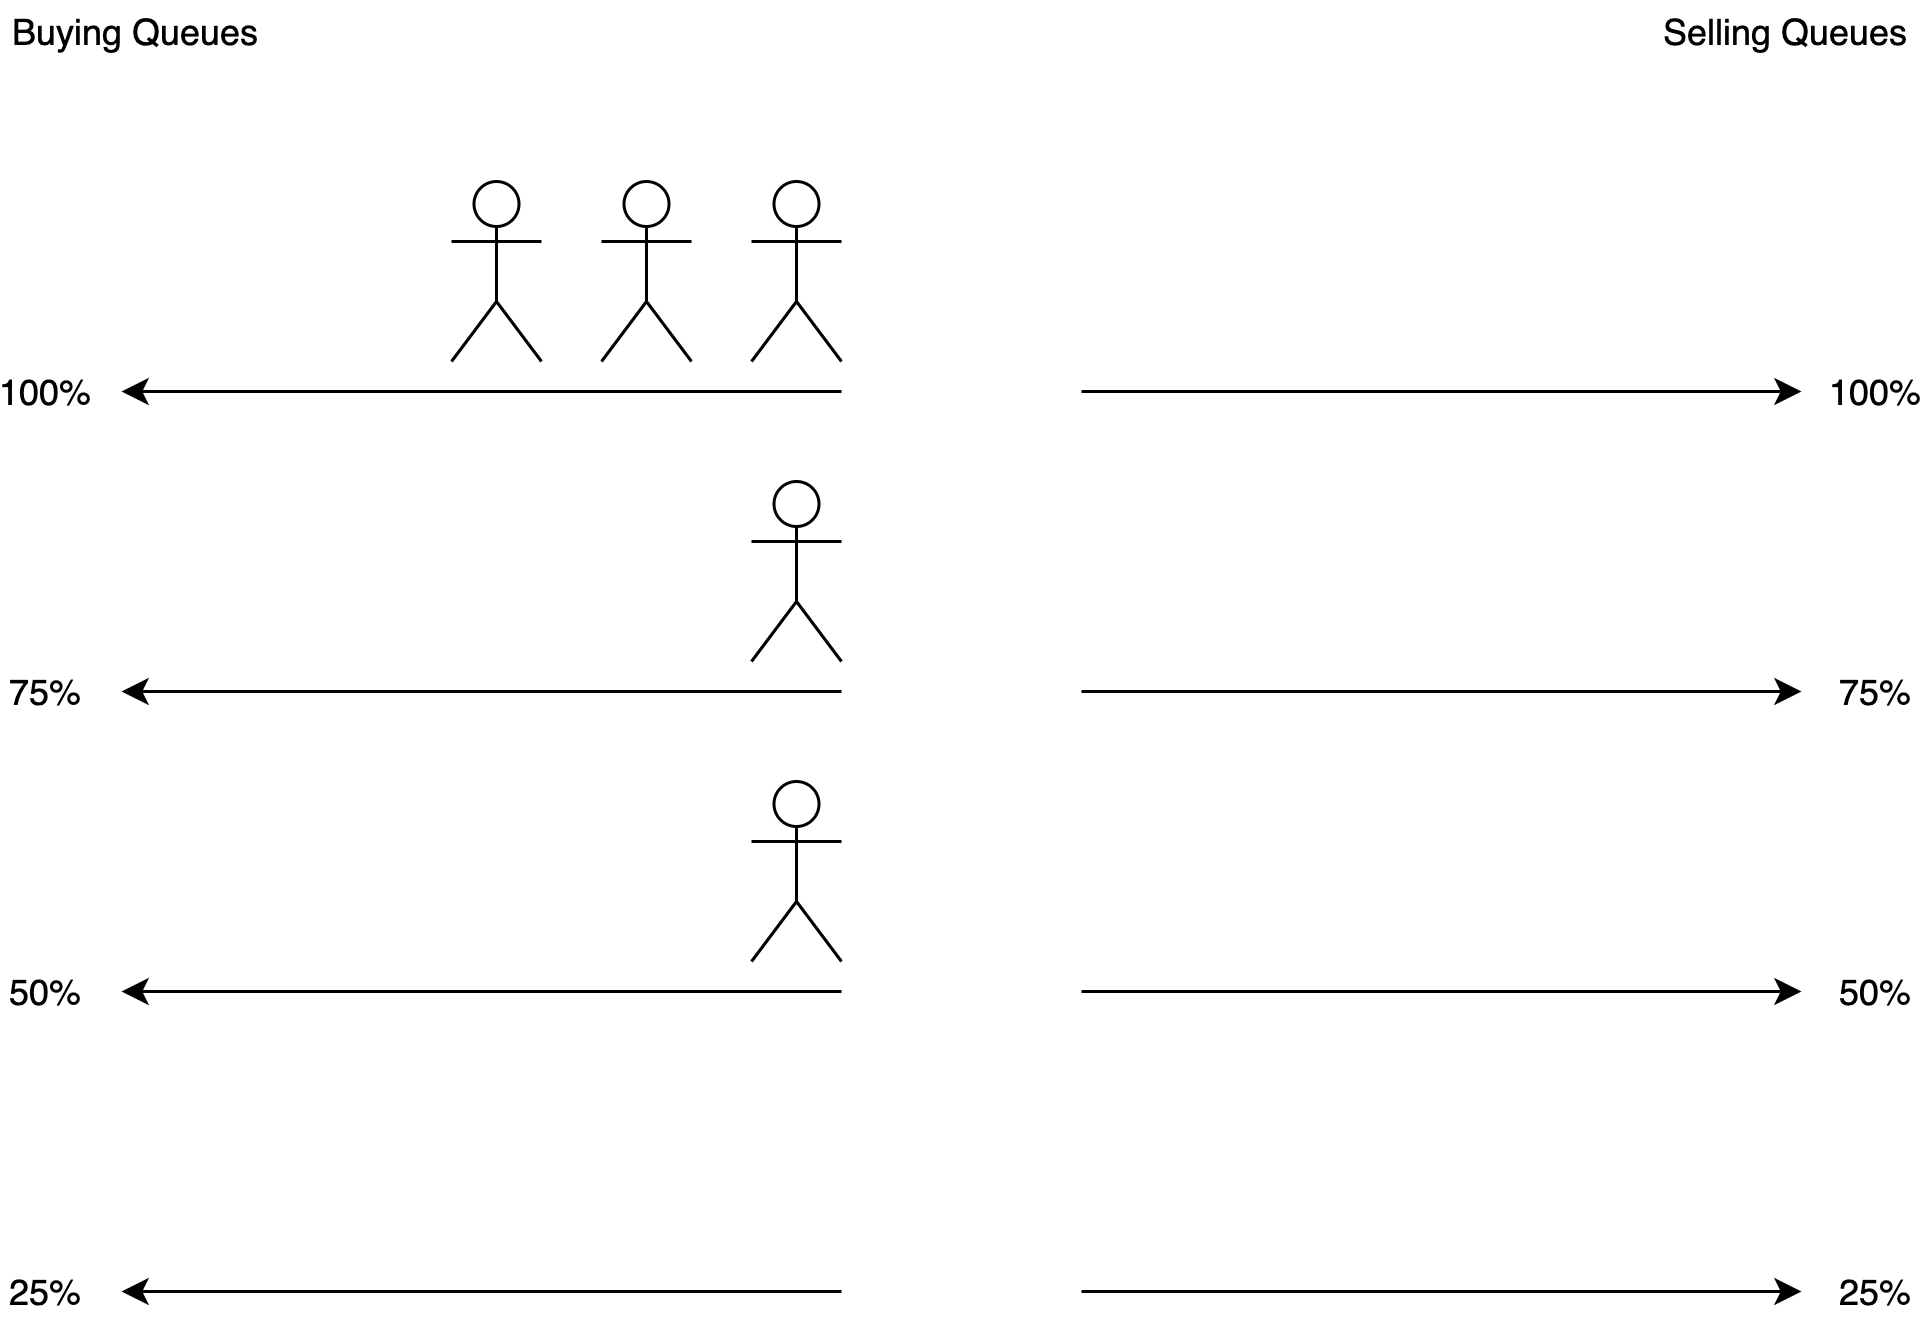
\includegraphics[width=16cm]{figures/aftermarket-high-demand.png}
    \caption{Aftermarket with high demand}
    \label{fig:aftermarket-high-demand}
\end{figure}

It is also possible that the aftermarket levels at a lower price than the original ticket price. This is shown in Figure \ref{fig:aftermarket-mixed} where multiple people are willing to sell the ticket for 75\% of the original price. On the other side, multiple people are willing to buy a ticket for only 50\% of the original ticket price. In this state, any seller could immediately settle a trade at 50\% of the original price and any buyer could immediately fill an offer at 75\%. 

\begin{figure}[H]
    \centering
    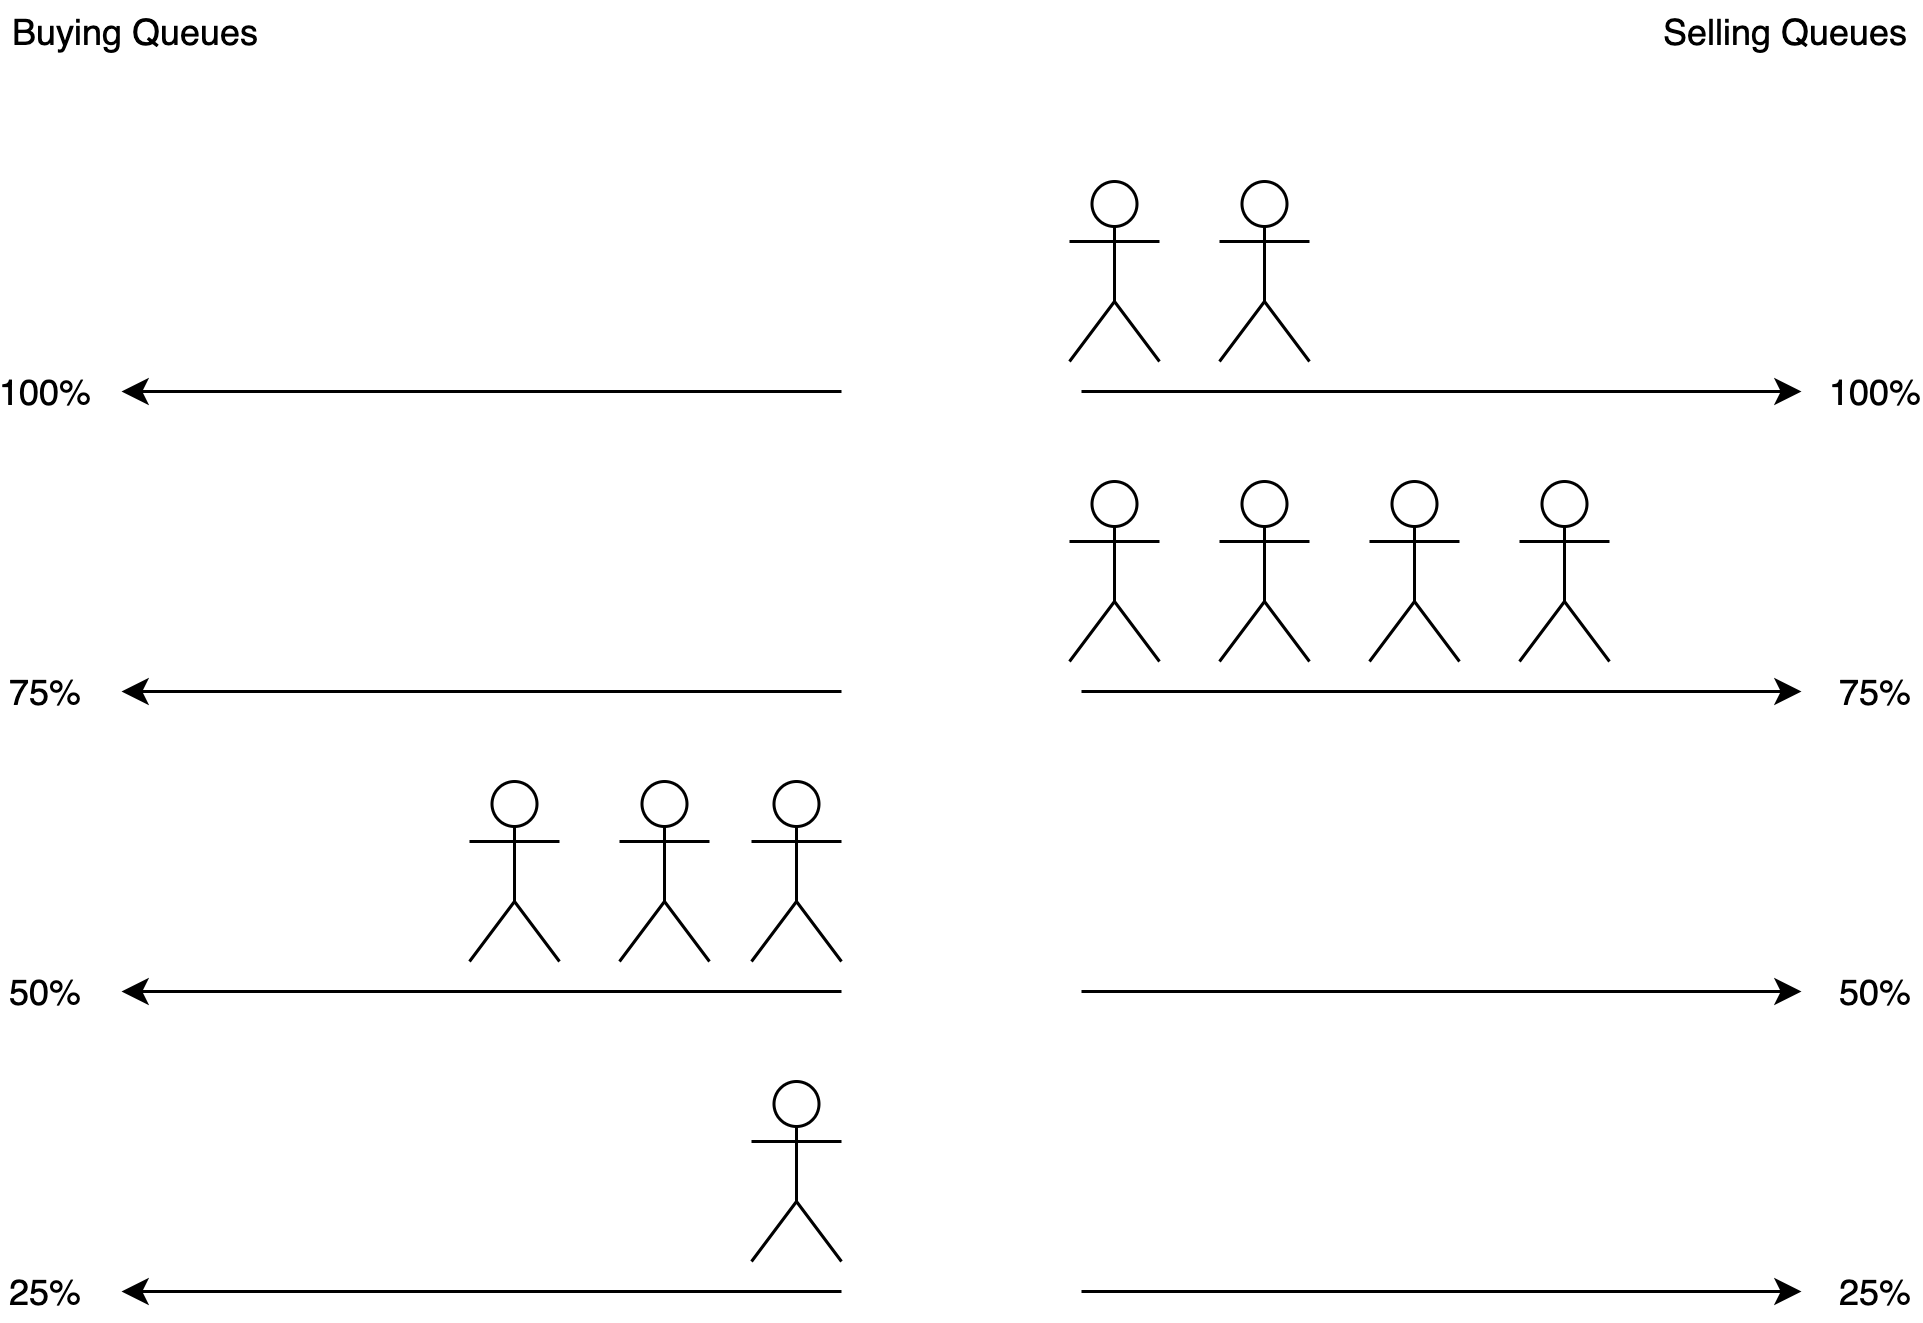
\includegraphics[width=16cm]{figures/aftermarket-mixed.png}
    \caption{Aftermarket with lower prices than original ticket price}
    \label{fig:aftermarket-mixed}
\end{figure}

Another scenario that is possible can occur when people join the wrong queue. This can occur when a sell an buy order is processed in the same block or due to wrong interaction with the smart contract. Such a state of the aftermarket is shown in Figure \ref{fig:aftermarket-arbitrage}. There is a person willing to sell a ticket for less highest offer on the buyer side. This opens the possibility of arbitrage trading. A third person can buy the ticket at 50\% and immediately resell the ticket again for 75\%. 

\begin{figure}[H]
    \centering
    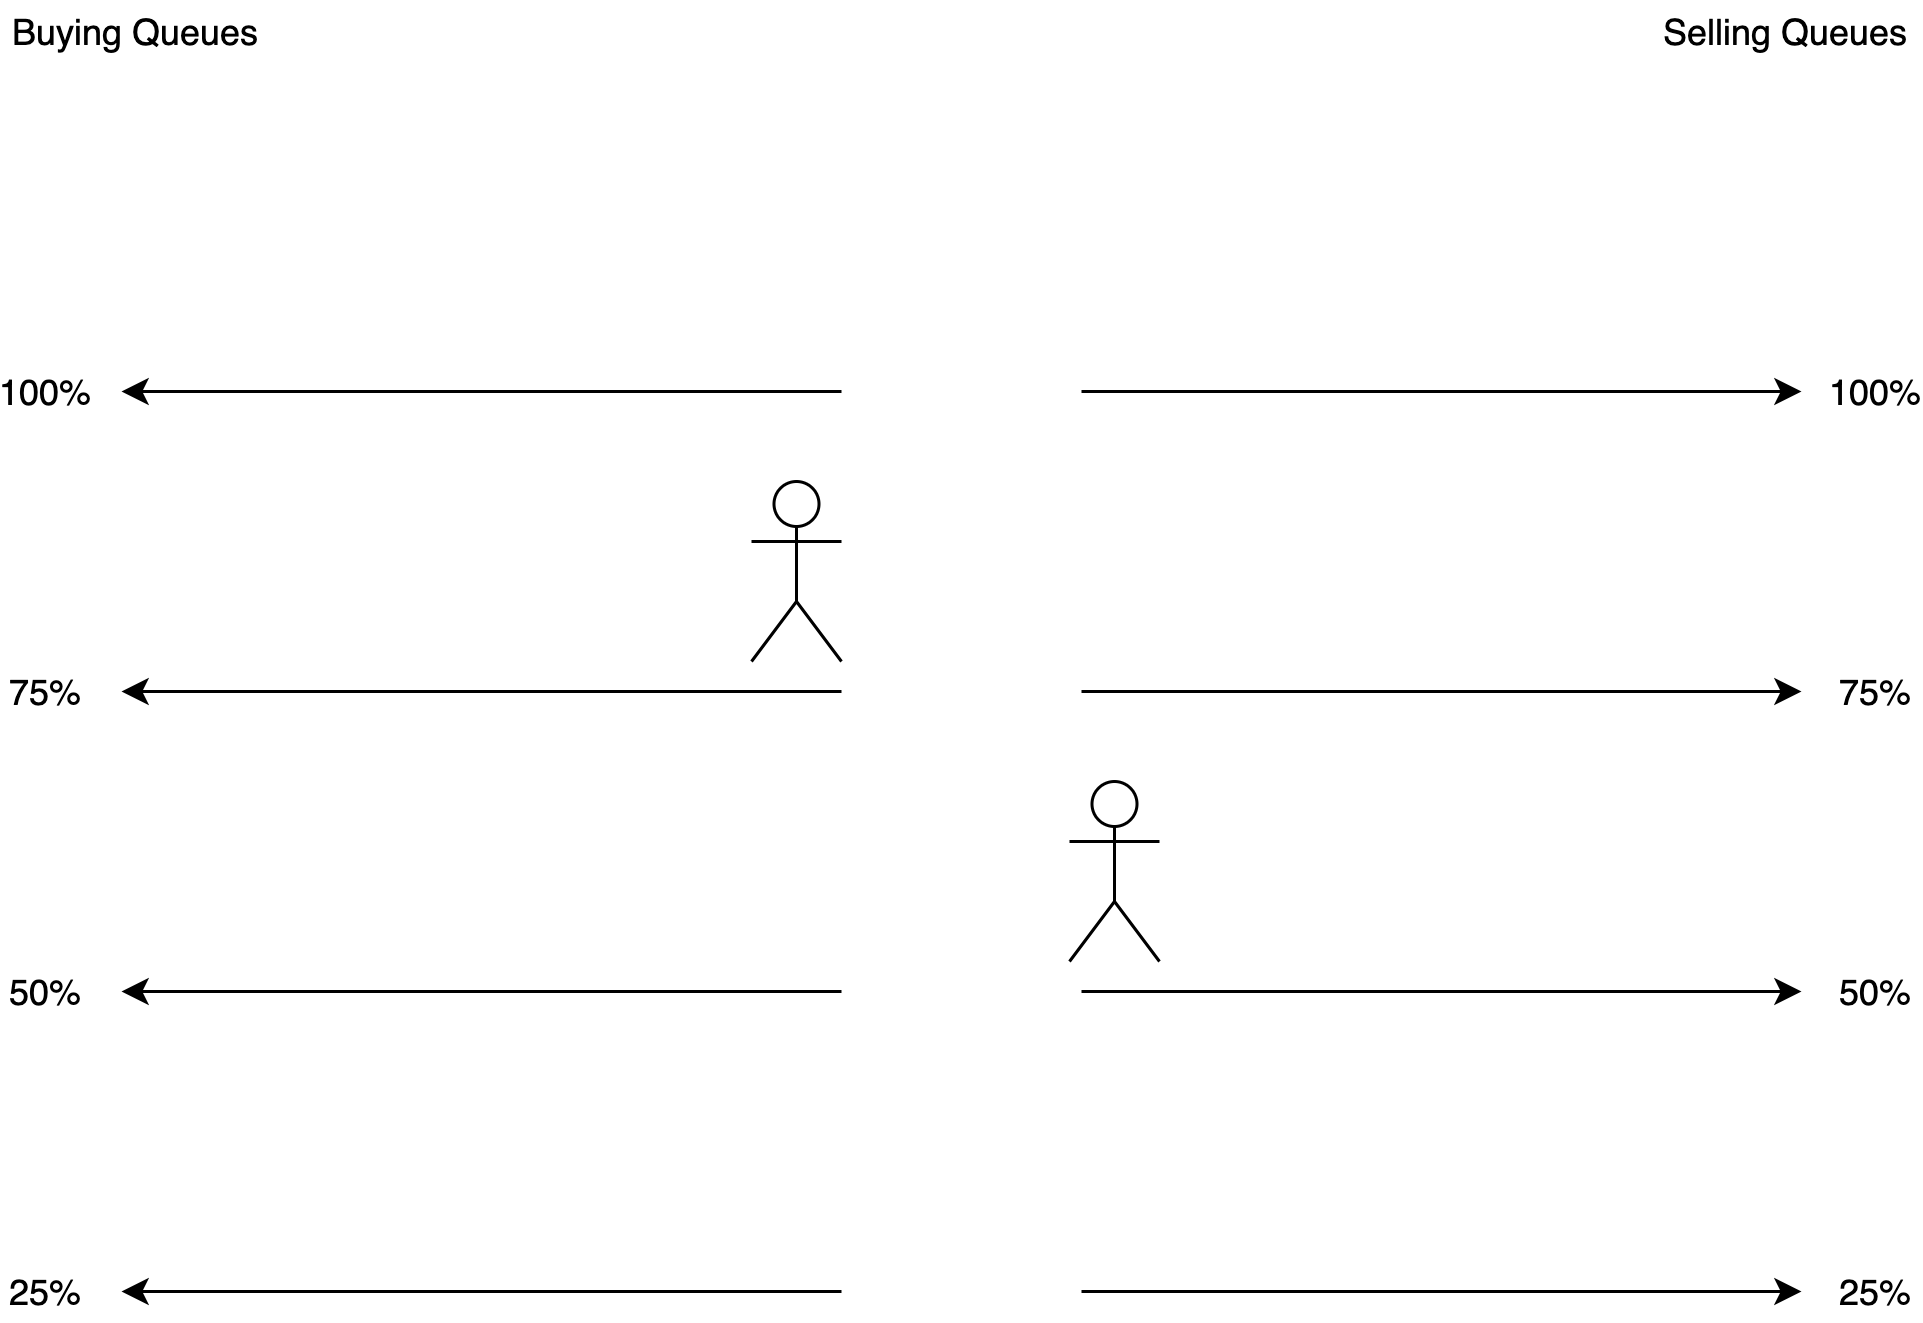
\includegraphics[width=16cm]{figures/aftermarket-arbitrage.png}
    \caption{Aftermarket with arbitrage opportunities}
    \label{fig:aftermarket-arbitrage}
\end{figure}

There are two solutions to solve that problem. Joining the wrong queue due to human error can be eliminated by warning the user in the frontend application that joining the selected queue results in a loss of opportunity cost. 

Solving the issue in the smart contract comes at the price of efficiency. Additional parameter can be introduced to keep track how many people are in each queue. Before each trade, the smart contract evaluates if the described state occurs. However, depending on the granularity of the queues, it might not be feasible to loop over each queue as this results in higher network fees and might lead to an 
\textit{out-of-gas exception}.

In this project, the ... solution was chosen.

\section{ERC standard}
All three ERC standard explained in Section \ref{subsubsection:token-interfaces} require a function which allows the owner to transfer the token/ticket to another address of his choice. Without explicitly deactivating this function, people are to sell the ticket on a different platform for higher prices and consequently, allowing a secondary market to emerge. The goal of this project is that there exists only one marketplace/exchange for each event operating transparently on the blockchain. Also, tickets must not transferred in the same way as these ERC standards do.

It is be possible to deactivate the transfer function or whitelist a specific exchange address such that tickets could only be sold through this exchange. However, this breaks the design principle of these standards. These standards were developed to create a common interface such that a token can be used across multiple exchanges and the usability is the same among different tokens. Also, tickets must only be resold in one contract to minimize the risk of emerging a black market (as described in Section \ref{section:aftermarket}). Merging the event logic with the aftermarket logic in one contract has a positive side-effect that no extra transaction is needed to approve the DEX (aftermarket). 

Furthermore, The logic for approving and storing other exchanges increases the complexity of the event smart contract and becomes more expensive to create deploy a new event.

These are the reason why an event contract does not implement and of the ERC standard interfaces and is bundled as one contract. 
\section{Presale}\label{section:des:presale}
Whenever an event takes place and the demand for the tickets is high, the potential guests will all try to buy the tickets when the sale period starts. This leads to a high traffic on the ticket sellers website. It it is then also not clear, which person can finish the buying process and is often determined by the quality of their internet provider.

To prevent this problem and have fair and clear odds for every potential guest, it was decided to use a lottery system for the initial sale of the tickets. Every guest, that wants to attend the event, can place a buy order in the presale. This order will cost as much as the ticket. At the end of the presale period, the tickets will be distributed using a random number, In the case a guest has not won a ticket, he then will be abke to reclaim the spend money. If there are more tickets than guest in the presale, everybody will get a ticket. 

 A guest will only be able to place a single buy order for only one ticket, since a fair lottery for multiple tickets is not possible on the blockchain. 

random number
ring model
why only one ticket? kgm not possible, could not find a solution with fair distribution


% author: Simon Bachmann

\section{Social Trust Certificates}\label{section:social-trust-certificates}

A decentralized ticketing platform does not restrict any user from creating an event on the DL. Thus, a mechanism must be developed to mitigate fraudulent events.

A common design pattern for this problem is an on-chain voting mechanism as explained in Section \ref{section:blocktix}. Usually, these decentralized platforms create a multi-purpose token for this. One of the tokens functions is governance. Token holders are eligible to cast votes if they think an event is fraudulent and in return they receive maintenance fees. However, this requires that the event creator must deposit some currency when creating an event. Furthermore, people must make an on-chain transaction to vote on suspicious events. This makes the UX more complex for the event host. Introducing a new token for every decentralized app also results in a fragmented ecosystem.

The goal is to enable users to check whether an event is legitimate or not without the need of a governance mechanism. Furthermore, the level of trust that is needed from third parties must not be greater than in the current ticketing ecosystem. 

\textit{Social trust certificates} enable a user to check whether the event is legitimate or not without the need of a third party. Event hosts upload the same public key, that is used for creating the event, to a social profile or the official event website. This way, an event host can proof his ownership of the event as well as the social profile or website. 

Event guests can retrieve the URL of the website or social profile from the SC and then verify themselves, if the event is legitimate or not. However, this is not 100\% foolproof. For an imposter it is easy to fake an official website with a slightly different URL and buy followers on social media platforms. However, this threat already exists today. Aggregating multiple social media platforms makes it harder for an attacker and thus, increases the legitimacy of an event compared to today's standards. 

Figure \ref{fig:trust-certificate-event-website} illustrates how the event host can use the official event website to increase the authenticity of the event. 

\begin{figure}[H]
    \centering
    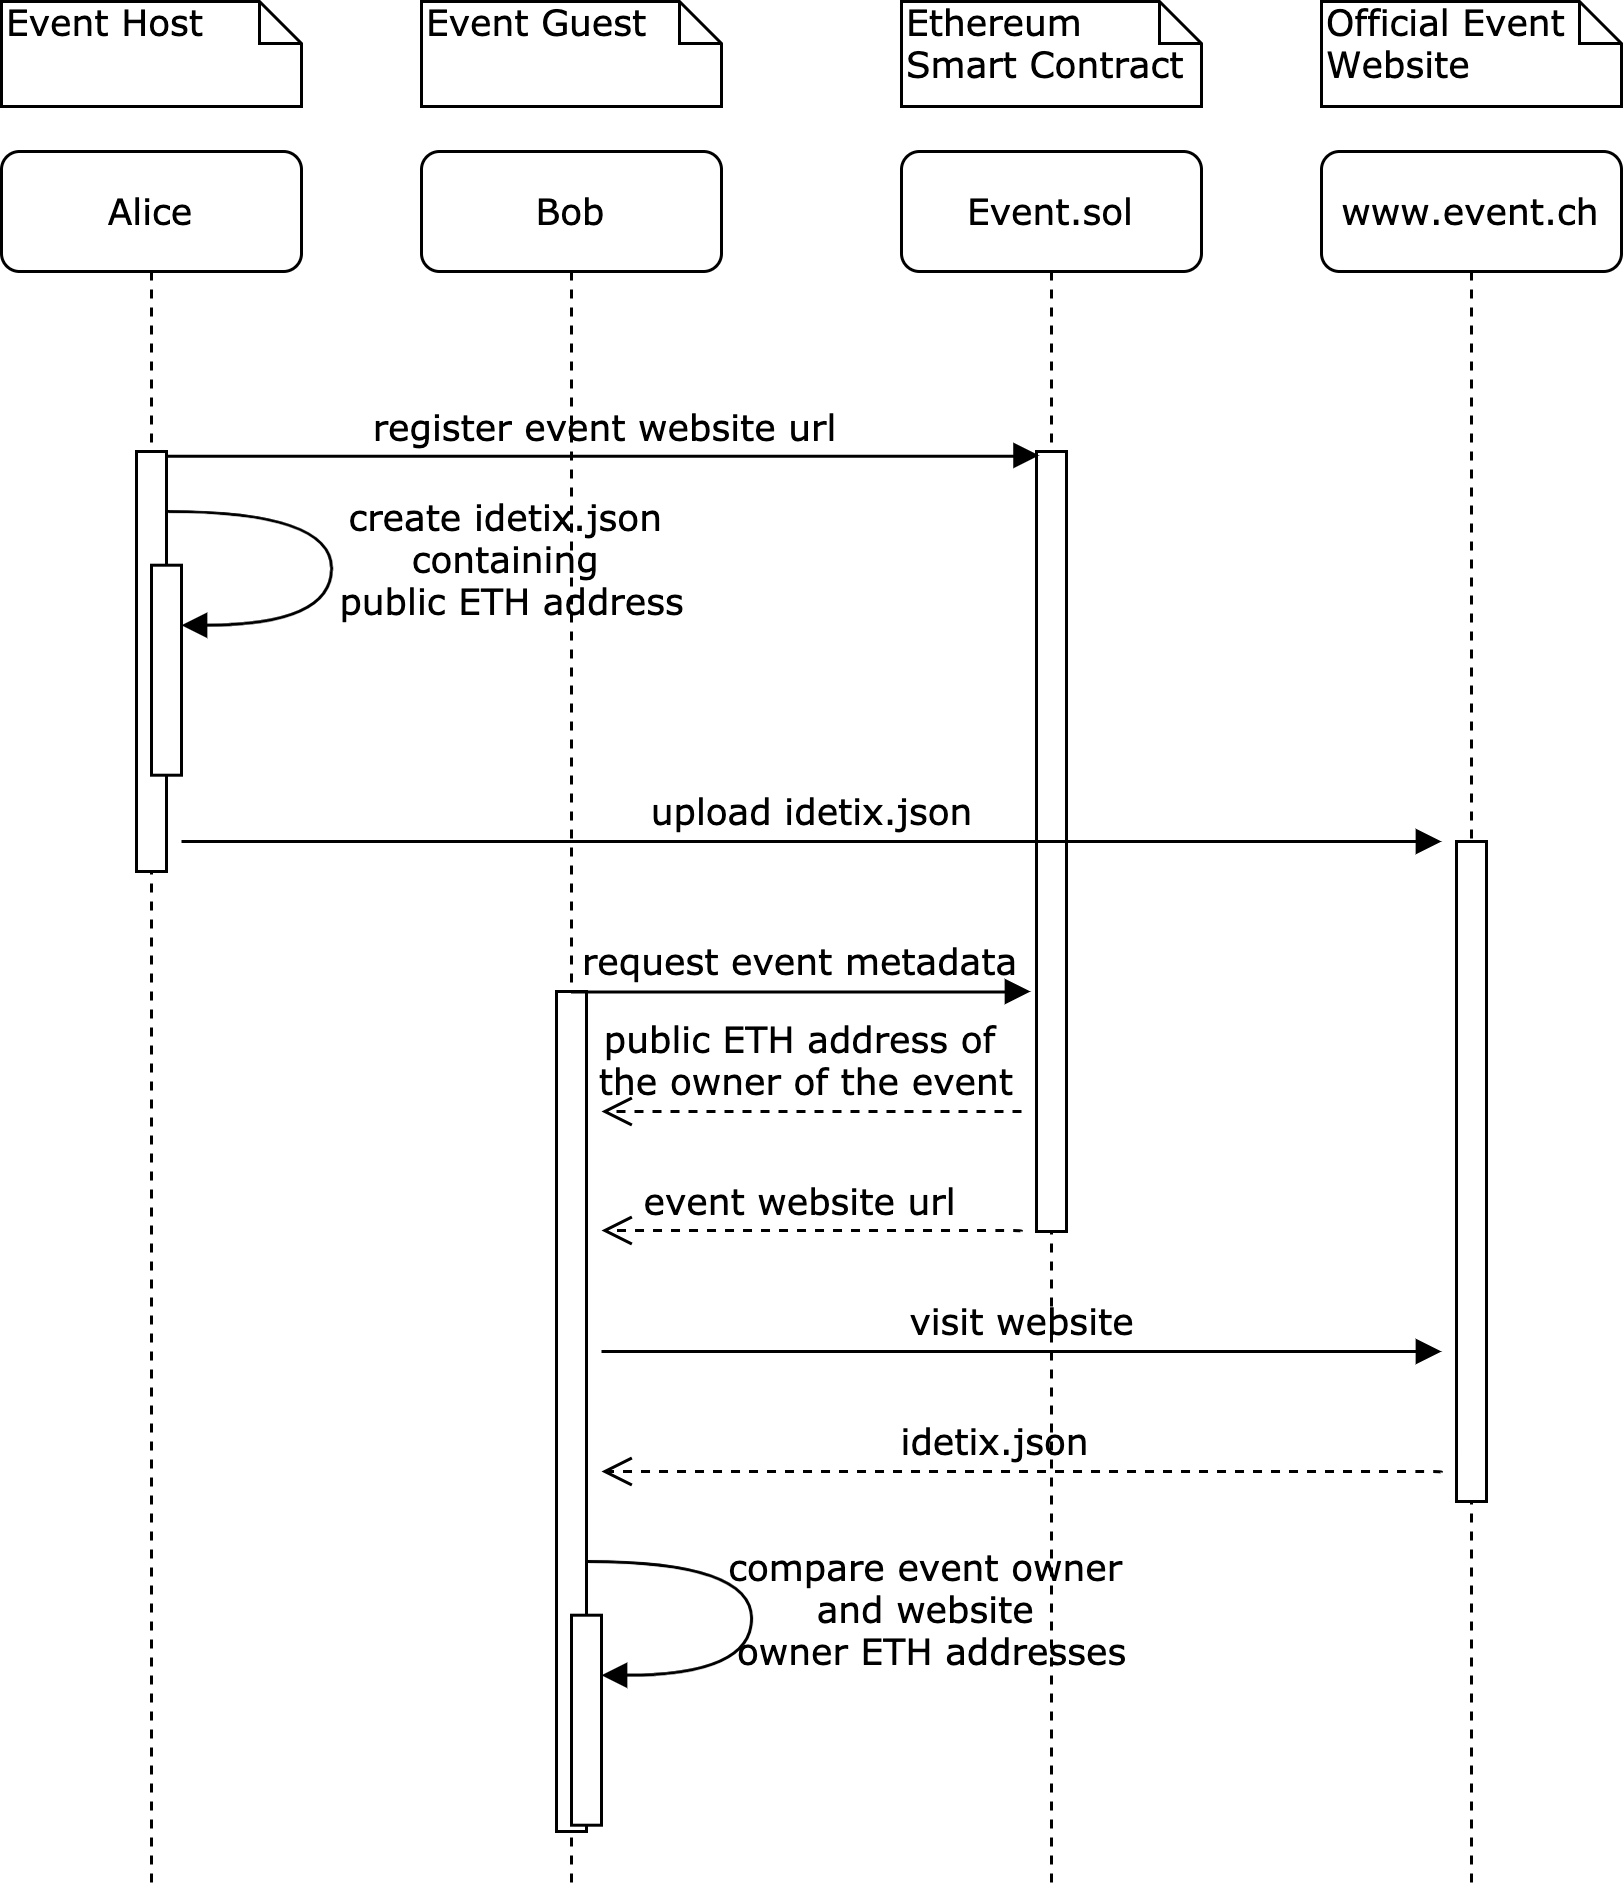
\includegraphics[width=14cm]{figures/social-trust-certificates.png}
    \caption{Social trust certificated on the event website}
    \label{fig:trust-certificate-event-website}
\end{figure}

Similarly, this procedure can be applied to any social profile such as Twitter, Facebook, Instagram and other social media platforms. Instead of uploading a JSON file or HTML meta-tag to the website, the public address is included in the profile description on that particular social media platform. 
\section{Access Control}\label{section:access-control}



\begin{figure}[H]
    \centering
    \includegraphics[width=14cm]{design/diagrams/AcessControl.png}
    \caption{Access Control Sequence Diagram}
    \label{fig:access-controll}
\end{figure}

As the Guest wants to gain access to the event, he is confronted with the access control. As the ticket is linked to the ethereum address of the guest, he just have to proof the ownership of the given ethereum address. In order to do this, following system is proposed.

The access control terminals are registered at the back end. Every terminal gets its unique identifier. The terminal then requests an unique random sequence, which is stored with the corresponding terminal id in the back end. This random sequence is then displayed alongside the back end URL as a QR-code on the terminal. The guest reads the QR-Code and extracts the random sequence. He then proceeds to sign the sequence using his ethereum address proofing his ownership. The signature, the ethereum address and the random sequence are then sent to the back end. There, the validity of the signature is evaluated, it is checked, whether the random sequence exists and the block chain is queried, to check, whether the ethereum address actually holds a ticket. It is also checked, whether this ticket already entered the venue. When all these checks are successful, the terminal, specified by its id, is messaged to let the guest pass. At the same time, the ethereum address and the corresponding ticket are added to the database, that tracks the area the ticket owner are in (Area Control).


%\input{.tex}
%\input{.tex}
\chapter{Evaluation}\label{chapter:evaluation}
\chapter{Summary}\label{chapter:summary}

%/ \begin{thebibliography}{99}
\addcontentsline{toc}{chapter}{Bibliography}

\bibitem{label} Autoren: Titel, Verlag, \url{http://...}, Datum.

\bibitem{blocktix-whitepaper} Florian Mathieu and Ryno Mathee: Blocktix: Decentralized Event Hosting and Ticket DistributionNetwork (white paper), \url{https://whitepaper.io/document/332/blocktix-whitepaper}, September 20 2017, accessed March 28 2020.


\bibitem{origin-protocol-whitepaper} Matthew Liu and Josh Fraser: Origin Protocol (white paper), \url{https://www.originprotocol.com/en/whitepaper}, December 26 2019, accessed March 28 2020.

\bibitem{blockparty-whitepaper} Blockparty: An Event Ticketing Blockchain Protocol (white paper), \url{https://cms.goblockparty.com/wp-content/uploads/2019/04/Blockparty-Event-Ticketing-Whitepaper-v-4.6.pdf}, May 2018, accessed March 31 2020.

\bibitem{metamask-breaking-changes} Erik Marks: Breaking Changes to the MetaMask Inpage Provider, \url{https://medium.com/metamask/breaking-changes-to-the-metamask-inpage-provider-b4dde069dd0a}, November 5 2019, accessed March 28 2020.

\bibitem{metamask-mobile} Jason Lee: MetaMask Mobile Beta — a feature guide and walkthrough, \url{https://medium.com/metamask/metamask-mobile-public-beta-a-feature-guide-and-walkthrough-9d01de7190ae}, July 23 2019, accessed March 28 2020.




\end{thebibliography}



\bibliographystyle{IEEEtranN}
\bibliography{bibliography}

\chapter*{Abbreviations}
\addcontentsline{toc}{chapter}{Abbreviations}
\markboth{ABBREVIATONS}{}


\abr{AAA}{Authentication, Authorization, and Accounting}
\abr{NPM}{Node Package Manager}
\abr{Metamask}{Browser plugin for interacting with the Ethereum blockchains}
\abr{tps}{Tickets per second}

\chapter*{Glossary}
\addcontentsline{toc}{chapter}{Glossary}
\markboth{GLOSSARY}{}


\begin{description}
  \item[Authentication] 
  \item[Authorization] Authorization is the decision whether an entity is allowed to perform a particular action or not, 
       e.g. whether a user is allowed to attach to a network or not.
  \item[Accounting]
\end{description}


\addcontentsline{toc}{chapter}{List of Figures}
\listoffigures
\addcontentsline{toc}{chapter}{List of Tables}
\listoftables

\appendix

\chapter{Installation Guidelines}





\end{document}
